\section{Considerações Iniciais}

Vimos que a acessibilidade em ambientes de aprendizagem é uma necessidade crescente na era digital, onde as TICs podem desempenhar um papel crucial ao tornar o conteúdos educacionais acessíveis a todos os alunos, independentemente de individualidades físicas ou sensoriais \cite{Mayer2021}. Nesse contexto, investigamos como o enriquecimento de OAs com transcrições/legendas automáticas podem aumentar a inclusão e o engajamento na educação \cite{FalvoJr2023_HICSS,FalvoJr2024_FIE}.

O conceito de OAs é central para as práticas pedagógicas atuais, uma vez que desempenham o papel de recursos digitais flexíveis que podem ser reutilizados para apoiar o processo de ensino-aprendizagem \cite{Parakh2022}. Com isso, a Arquitetura \textit{Speech2Learning} é nossa principal contribuição, através da qual propomos o aprimoramento de OAs audíveis por meio de ASR/STT, promovendo a geração automática de legendas, transcrições ou traduções. Assim, videoaulas podem ser acessíveis em diferentes línguas e até mesmo sinalizadas por avatares de línguas de sinais baseados em texto.

Este capítulo detalha a aplicação prática da \textit{Speech2Learning} por meio de dois Estudos de Caso, projetados como instâncias concretas da arquitetura. Esses estudos foram conduzidos em colaboração com a \textit{EdTech} brasileira DIO, que foi essencial para viabilizar avaliações empíricas em OAs de uma plataforma educacional real, marcando um passo significativo na direção de soluções mais acessíveis e inclusivas.

\section{Estudo de Caso 1: Legendas em Videoaulas}

Nosso primeiro Estudo de Caso buscou investigar a precisão dos principais serviços de ASR, uma vez que essa tecnologia é central na Arquitetura \textit{Speech2Learning}. Na prática, utilizamos um conjunto de recursos educacionais, disponíveis na plataforma de \textit{e-learning} da DIO, para a construção de uma \sigla{PoC}{Prova de Conceito} focada na transcrição e legendagem desses OAs através de serviços de ASR.

Sendo assim, o objetivo deste estudo é expandir nossa compreensão sobre o papel das transcrições e legendas automáticas para um processo de ensino-aprendizagem mais acessível. Para tal propósito, discutimos a convergência dos resultados quantitativos e qualitativos obtidos por meio das três fontes de dados distintas, uma estratégia oriunda da metodologia de triangulação de dados \cite{LimaJunior2021}.

Segundo \cite{Farquhar2020}, é possível explorar múltiplas fontes de evidências (quantitativas e/ou qualitativas) e discutir suas respectivas convergências por meio de uma abordagem de triangulação de dados. No contexto deste Estudo de Caso, as seguintes fontes foram observadas: (i) métodos de similaridade léxica; (ii) respostas de um \textit{Survey} anônimo; e (iii) estudos de uma pesquisa documental complementar.

Desta forma, as seções a seguir abordam desde a implementação da PoC junto a \textit{EdTech} DIO até os detalhes metodológicos e resultados obtidos. Com isso, desenvolvemos discussões e percepções muito interessantes sobre a importância e potencial de TICs como o ASR/STT na promoção de soluções educacionais mais acessíveis.

\subsection{Prova de Conceito: API REST para Legendar Videoaulas}

O desenvolvimento de uma PoC, primeira instância da \textit{Speech2Learning}, surgiu de uma necessidade de negócio da \textit{EdTech} DIO de legendar suas videoaulas de forma escalável. Para isso, uma API REST foi implementada para transcrever videoaulas curtas (entre 15 e 30 segundos), algo comum considerando o conceito de \textit{microlearning} adaptado pela DIO para suas necessidades educacionais. 

Com isso, foi possível explorar os padrões de metadados inerentes à Arquitetura \textit{Speech2Learning} e gerar transcrições e legendas para videoaulas em múltiplos idiomas. Nesse sentido, definimos o escopo da PoC aos idiomas suportados na plataforma da DIO: Português, Inglês e Espanhol. Desta forma, foi possível ampliar a acessibilidade desses OAs por meio de transcrições e legendas geradas automaticamente a priori.

Conforme o diagrama da \autoref{fig:chapter4-cs1-poc-diagram}, a API REST segue as diretrizes da \textit{Speech2Learning}, bem como apresenta uma visão da estrutura de C\&C \cite{Bass2021}. O esquema de cores dos componentes corresponde ao das camadas na \autoref{fig:chapter3-speech2learning-arch}, ilustrando uma implementação em conformidade com os limites lógicos/estruturais pré-definidos para uma API REST.

\begin{figure}[htb]
\centering
\caption{Visão 1ª Instância da \textit{Speech2Learning}: API REST para Legendar Videoaulas}
\label{fig:chapter4-cs1-poc-diagram}
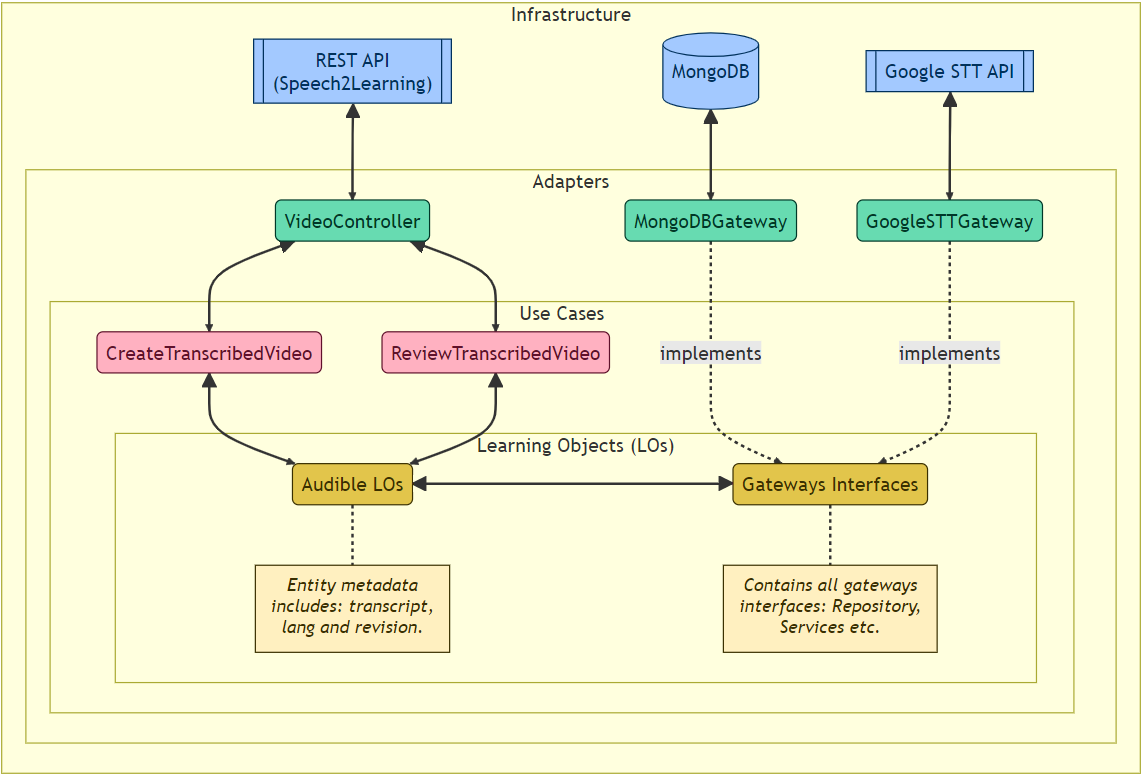
\includegraphics[width=\columnwidth]{images/chapter4-cs1-poc-diagram.png}
\fdireta{FalvoJr2023_HICSS}
\end{figure}

O diagrama define dois \textit{Casos de Uso} relacionados à transcrição de vídeos: \textit{Criar} e \textit{Revisar}. Esta visão é interessante pois esclarece as funcionalidades implementadas na PoC. Além disso, nossas entidades foram projetadas como \textit{OAs Audíveis}, uma vez que lidamos com videoaulas. Para concluir, detalhes sobre a implementação também são expostos claramente na camada de \textit{Infraestrutura}. Por exemplo, nosso ponto de entrada é uma \textit{API REST}, o \textit{MongoDB} é o banco de dados e \textit{Google STT API} (API externa) é o provedor de STT.

Para oferecer uma perspectiva mais técnica, a PoC pode ser consumida sob demanda através de uma requisição HTTP POST para uma API REST reativa. Este endpoint aciona um fluxo de trabalho assíncrono para extrair o áudio do vídeo, otimizando assim o consumo de largura de banda antes de invocar a \textit{Google STT API}. Após a resposta dessa requisição, a transcrição é armazenada nos metadados do \textit{OA Audível}, tornando essa transcrição automática elegível para revisão.

Para revisar a transcrição de um OA existente, basta fazer uma requisição HTTP PUT para atualizar este recurso, versionando suas transcrições por meio dos metadados. Vale lembrar que, a \textit{Speech2Learning} apenas define diretrizes para a criação de soluções baseadas em STT para promover a acessibilidade de OAs, sem impor decisões de design, tecnologias ou aspectos de segurança.

Na prática, o acesso à PoC foi restrito à Equipe de Educação da DIO, garantindo que seus OAs (videoaulas) fossem criados e revisados com segurança e em um ambiente controlado. Ressaltamos que as transcrições automáticas exigiram uma extensa revisão por especialistas em línguas da empresa, destacando a necessidade de otimizar o processo de transcrição e explorar outros serviços de STT.

Inspirados pelos \textit{insights} e desafios desta PoC, pensamos em expandir nossas percepções por meio de um Estudo de Caso mais amplo. Por sua vez, esta iniciativa de investigação visa analisar mais profundamente as nuances entre diferentes provedores de STT. Portanto, para nosso Estudo de Caso, selecionamos 15 videoaulas cujas transcrições foram revisadas por especialistas em idiomas da DIO durante a PoC. Esta quantidade e duração de vídeos foram estrategicamente definidas para controle financeiro (custo dos provedores de STT) e, principalmente, viabilizar um \textit{Survey} coeso para avaliação da precisão das transcrições automáticas sob novas perspectivas.

Para uma análise mais robusta, procuramos diversificar as línguas e os professores das videoaulas, de forma a captar diferentes sotaques e regionalidades. A \autoref{tab:chapter4-poc-audios-summary} detalha as características linguísticas e técnicas dos áudios extraídos das videoaulas. Este conjunto diversificado de dados servirá como referência, nos permitindo analisar criticamente o desempenho de outros fornecedores de STT em múltiplos contextos de ensino-aprendizagem.

\begin{table}[htb]
\centering
\caption{\textit{Dataset} do Estudo de Caso 1 (Áudios Extraídos das Videoaulas)}
\label{tab:chapter4-poc-audios-summary}
\begin{tabular}{|c|c|c|c|l|c|}
\hline
\textbf{ID} & \textbf{Língua} & \textbf{Sotaque} & \textbf{Gênero} & \textbf{Tópico Educacional} & \textbf{Tempo} \\ \hline
1 & pt-BR & BRA & M & Apps Android & 0:17 \\ \hline
2 & pt-BR & BRA & M & SCRUM & 0:26 \\ \hline
3 & pt-BR & BRA & F & Selenium WebDriver & 0:23 \\ \hline
4 & pt-BR & BRA & F & Blockchain & 0:20 \\ \hline
5 & pt-BR & BRA & M & Kernel Híbrido & 0:24 \\ \hline
6 & en-US & BRA & F & Visto de Trânsito & 0:29 \\ \hline
7 & en-US & USA & Ambos & Entrevista de Emprego & 0:16 \\  \hline
8 & en-US & BRA & F & Oportunidades de Emprego & 0:20 \\  \hline
9 & en-US & BRA & F & Liderança Servidora & 0:15 \\  \hline
10 & en-US & BRA & M & Goroutines & 0:15 \\  \hline
11 & es-AR & ARG & F & Lógica de Programação & 0:12 \\  \hline
12 & es-AR & ARG & F & Linguagens de programação & 0:21 \\  \hline
13 & es-AR & ARG & F & Tipos de Dados em Python & 0:14 \\  \hline
14 & es-AR & ARG & F & Hello World com Python & 0:17 \\  \hline
15 & es-AR & ARG & F & String Slicing com Python & 0:26 \\ \hline
\end{tabular}
\fadaptada{FalvoJr2023_HICSS}
\end{table}

Este conjunto de dados (\textit{dataset}) passou por um rigoroso controle de qualidade de áudio, protocolo padrão para todo conteúdo oferecido na plataforma educacional da DIO. Para garantir a transparência dessas informações, disponibilizamos uma pasta pública\footnote{\textit{Dataset} do Estudo de Caso 1: \url{https://bit.ly/S2L-Audios}} que contém todas as amostras de áudio suas respectivas transcrições revisadas por especialistas em línguas da DIO. 

Tecnicamente, o \textit{dataset} atende ou excede os seguintes critérios de qualidade: canais de áudio duplos, taxa de amostragem de 44,1 kHz e precisão de 16 bits. Tais aspectos técnicos não só garantem excelente qualidade de som, mas também contribuem para transcrições automáticas mais precisas.

Nesse contexto, a realização de um Estudo de Caso é uma excelente opção para ampliar esta PoC e orientar análises e discussões mais profundas. Resumidamente, a PoC identificou a necessidade de reduzir o retrabalho exigido na revisão das transcrições automáticas e assim melhorar a eficiência do processo de transcrição. Esta progressão da PoC para um Estudo de Caso reflete uma abordagem comum em pesquisa que permite o desenvolvimento iterativo \cite{Runeson2009}. 

O \textit{dataset} compilado nesta PoC nos permitiu analisar a qualidade das transcrições automáticas em vários provedores de STT, usando as transcrições de referência revisadas pelos especialistas em idiomas da DIO como um controle confiável. A metodologia definida para o Estudo de Caso decorrente desta PoC, bem como seus resultados são apresentados a seguir.

\subsection{Metodologia}

Esta seção descreve a metodologia deste Estudo de Caso, com o objetivo de investigar o papel do ASR e do STT na melhoria da acessibilidade de OAs. Trata-se de uma investigação empírica, apoiada em raciocínio indutivo e pesquisa de campo. Ao contrário dos estudos experimentais, os Estudos de Caso reúnem informações de diversas fontes por meio de diferentes técnicas de coleta de dados \cite{Sommerville2015}.

Como dito anteriormente, firmamos uma parceria com a \textit{EdTech} DIO, que compartilhou conosco videoaulas disponíveis em seu currículo, oferecendo uma oportunidade de conexão entre a indústria e nossa pesquisa. A DIO concedeu acesso a parte de sua infraestrutura em nuvem, além de disponibilizar especialistas em línguas que revisaram os resultados do ASR durante a PoC. Esse processo de revisão foi fundamental para que as fontes de evidência, baseadas na precisão das transcrições e legendas de videoaulas, tivessem referências sólidas para nossas comparações e análises.

Como consequência, tanto os dados de similaridade léxica quanto as respostas do \textit{Survey} avaliaram o mesmo conjunto de 15 videoaulas: 5 em inglês, 5 em português e 5 em espanhol. Essa abordagem facilitou a obtenção de duas perspectivas quantitativas distintas sobre a qualidade das transcrições automáticas: uma derivada de algoritmos de similaridade léxica e a outra baseada nas percepções dos aprendizes.

Adicionalmente, nossa metodologia integra um terceiro aspecto de coleta de dados através de uma pesquisa documental focada em ASR/STT, além de aplicar a Teoria Fundamentada \cite{Charmaz2009} para assegurar um processo de análise de conteúdo. Portanto, nossa pesquisa documental visa fornecer dados qualitativos sobre o fenômeno observado \cite{LimaJunior2021}.

Ao triangular os dados coletados de similaridade léxica, das respostas do \textit{Survey} anônimo e da pesquisa documental complementar (\autoref{fig:chap4:triangulation-sources}), buscamos oferecer uma compreensão abrangente dos desafios e oportunidades associados à utilização de tecnologias ASR para aumentar a acessibilidade de OAs no domínio educacional. 

\begin{figure}[htb]
\centering
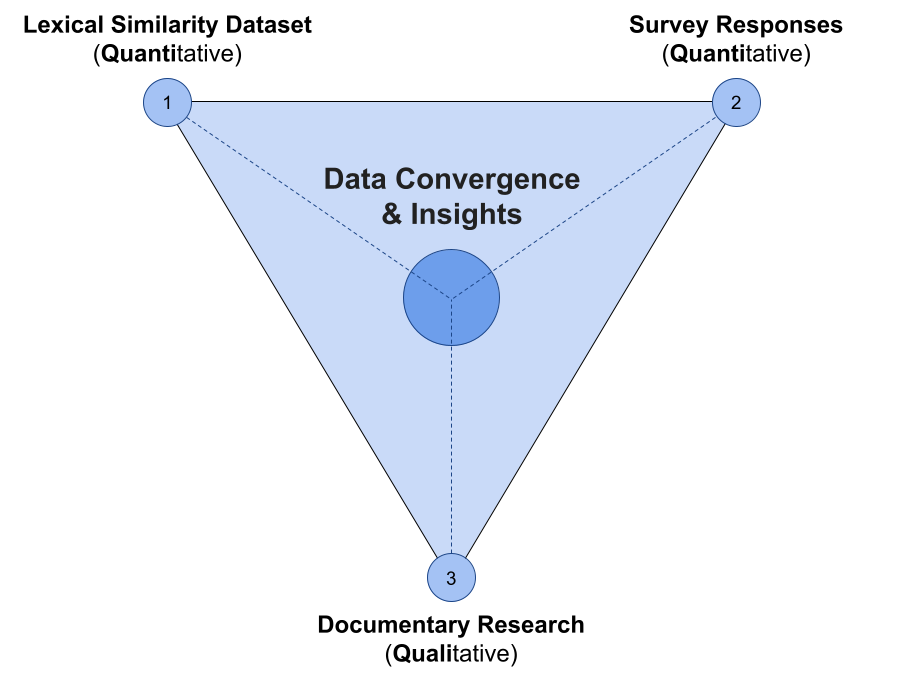
\includegraphics[width=0.75\textwidth]{images/chapter4-cs1-triangulation-sources.png}
\caption{Triangulação de Dados: Fontes de Evidência.}
\label{fig:chap4:triangulation-sources}
\fdireta{FalvoJr2024_FIE}
\end{figure}

A seguir, delineamos cada fonte de evidência e suas técnicas de coleta, esclarecendo todo o processo de triangulação e sua contribuição para uma compreensão robusta do impacto das tecnologias ASR, como o STT, na acessibilidade educacional.

\subsubsection{1ª Fonte de Evidência: Métodos de Similaridade Léxica}

Esta seção apresenta a metodologia definida para a primeira fonte de evidências da triangulação de dados, onde métodos de similaridade léxica têm como objetivo avaliar e identificar o provedor de ASR/STT mais assertivo para transcrição automática. Nesse sentido, algoritmos de similaridade léxica são métricas particularmente relevantes para a avaliação da precisão de transcrições automáticas, conforme discutimos detalhadamente em \citeonline{FalvoJr2023_HICSS}.

Medir a semelhança entre textos é uma prática comumente investigada em pesquisas acadêmicas, em geral apoiada por métodos de análise/similaridade léxica \cite{Majumdar2022}. Para comparar nossas transcrições automáticas e de referência, precisamos definir como extrairemos nossos dados quantitativos utilizando técnicas de similaridade léxica. No nosso contexto, algumas das alternativas mais interessantes são:

\begin{itemize}

\item \textbf{\sigla{CS}{Similaridade de Cosseno}}: Esta métrica é usada para medir a similaridade entre dois vetores. Especificamente, ela mede a semelhança na direção ou orientação dos vetores, ignorando as diferenças na sua magnitude ou escala. Ambos os vetores devem pertencer ao mesmo espaço de produto interno, o que significa que devem produzir um escalar ao multiplicar o produto interno. A similaridade de dois vetores é medida pelo cosseno do ângulo entre eles. A métrica CS varia de 0 a 1, onde um valor mais próximo de 0 indica menor similaridade e um valor mais próximo de 1 indica maior similaridade \cite{cosseno-1,cosseno-2,cosseno-3}.

\item \textbf{\sigla{JI}{Índice de Jaccard}}: Esta métrica é definida como a interseção de dois conjuntos de dados dividida pela união desses conjuntos, medindo a similaridade entre eles. No contexto de textos, pode ser expressa como o número de palavras comuns dividido pelo número total de palavras nos dois textos ou documentos. O JI varia de 0 a 1, onde 0 significa nenhuma similaridade e 1 significa sobreposição completa. O JI é calculado dividindo o número de observações em ambos os conjuntos pelo número de observações em cada conjunto, ou seja, o tamanho da interseção dividido pelo tamanho da união de dois conjuntos \cite{Majumdar2022,jaccard-1,jaccard-2}.

\item \textbf{\sigla{LD}{Distância de Levenshtein}}: Esta métrica de \textit{string} mede a diferença entre duas strings. Basicamente, a LD entre duas palavras é o número mínimo de edições de um único caractere (inserções, exclusões ou substituições) necessárias para transformar uma palavra na outra. Seu nome é uma homenagem a Vladimir Levenshtein, que considerou essa distância em 1965. A comparação LD é geralmente realizada entre duas palavras, determinando o número mínimo de edições necessárias para alterar uma palavra para outra. Quanto maior o número de edições, maior a diferença entre os textos. Uma edição é definida como a inserção, exclusão ou substituição de um caractere \cite{levens-1,levens-2}.

\end{itemize}

Neste estudo, aplicamos os três métodos mencionados, destacando sua relevância em nossa metodologia. Primeiramente, geramos e revisamos as transcrições de referência usando a instância da \textit{Speech2Learning}, desenvolvida como uma PoC. Em seguida, transcrevemos automaticamente cada OA utilizando diferentes serviços de ASR/STT, permitindo a comparação entre as transcrições de referência e as automáticas. Dessa forma, utilizamos os métodos de similaridade léxica CS, JI e LD como métricas de precisão.

Para essa finalidade, identificamos os principais provedores de ASR/STT baseados em IA do mercado \cite{Gartner2023}: Amazon, Google, IBM, Microsoft e OpenAI. Ademais, em colaboração com a DIO, garantimos que todos os OAs e suas transcrições de referência estavam devidamente revisadas e disponíveis no \textit{dataset} deste Estudo de Caso (\autoref{tab:chapter4-poc-audios-summary}).

Com os áudios otimizados do \textit{dataset}, integramos os serviços de ASR/STT de cada provedor e geramos suas respectivas transcrições automáticas. Para uma implementação organizada e documentada, utilizamos o Google Colab, detalhando todo o processo em um notebook público\footnote{Colab Notebook - Transcrições Automáticas com ASR/STT: \url{https://bit.ly/S2L-STTServices}}. De forma similar, comparamos as 15 transcrições automáticas com as transcrições de referência usando os três métodos de similaridade léxica (CS, JI e LD) em um segundo notebook\footnote{Colab Notebook - Algoritmos de Similaridade Léxica: \url{https://bit.ly/S2L-CaseStudy}}.

\subsubsection{2ª Fonte de Evidência: Respostas do \textit{Survey}}

Conduzimos um \textit{Survey} para avaliar as percepções dos alunos sobre a qualidade das transcrições automáticas fornecidas por ASR/STT. Esta pesquisa, que contou com 56 respostas, coletou \textit{feedbacks} quantitativos e qualitativos de participantes com experiência em tecnologia e educação. Disponibilizamos as respostas (\url{https://bit.ly/S2L-SurveyResponses}) e uma cópia do formulário (\url{https://bit.ly/S2L-Survey}) para que os dados e a dinâmica de preenchimento sejam completamente compreendidos.

O \textit{Survey} utilizou uma combinação de perguntas de escala Likert e perguntas abertas. As perguntas de escala Likert visavam avaliar quantitativamente a coerência das transcrições automáticas em três idiomas (inglês, português e espanhol). Esta estratégia nos permitiu uma análise cruzada entre as avaliações técnicas/léxicas e as centradas no usuário. As perguntas abertas buscavam obter \textit{insights} qualitativos sobre a eficácia percebida das soluções de ASR. No entanto, devido à conformidade ética, não exploraremos os dados qualitativos neste estudo.

Os participantes avaliaram as transcrições do mesmo conjunto de 15 videoaulas (cinco por idioma) e dos mesmos cinco provedores (Amazon, Google, IBM, Microsoft e OpenAI) utilizados no estudo de similaridade léxica. Este alinhamento entre as duas fontes garantiu que as Respostas do Survey complementassem diretamente a análise técnica de similaridade léxica, proporcionando uma visão holística do desempenho das transcrições.

Para mitigar vieses, os provedores foram anonimizados e receberam um identificador numérico aleatório em vez de serem nomeados, garantindo que as avaliações refletissem experiências genuínas dos usuários, sem influência do reconhecimento da empresa/marca. Esta abordagem metodológica está alinhada às melhores práticas em metodologia de pesquisa empírica, conforme defendido por \cite{Sommerville2015}, especialmente na coleta de \textit{feedbacks} e percepções dos usuários em estudos de engenharia de software.

\subsubsection{3ª Fonte de Evidência: Pesquisa Documental}

Para contextualizar e enriquecer nossos dados quantitativos, realizamos uma revisão de literatura que complementa nossos achados empíricos, identificando estudos relevantes sobre tecnologias ASR e STT. Esta revisão proporciona uma compreensão mais profunda do potencial e das limitações das tecnologias atuais baseadas em ASR.

Empregamos a \textit{Grounded Theory}, ou \sigla{TFD}{Teoria Fundamentada nos Dados}, como um \textit{framework} orientador para nossa análise documental. A TFD é uma metodologia sistemática e rigorosa utilizada na pesquisa qualitativa para desenvolver teorias emergentes diretamente dos dados \cite{Charmaz2009}. Diferentemente de abordagens que partem de hipóteses preconcebidas, a Teoria Fundamentada nos Dados permite a descoberta de temas e padrões de maneira indutiva, por meio de um processo iterativo de coleta e análise de dados.

Neste estudo, utilizamos a TFD para examinar os estudos selecionados na pesquisa documental. Este processo incluiu a codificação aberta dos dados, a identificação de temas recorrentes e a integração desses temas em uma teoria coesa. Assim, garantimos que nossas conclusões fossem baseadas diretamente nas evidências coletadas, sem impor noções preconcebidas.

Nossa pesquisa documental envolveu uma revisão complementar da literatura, incluindo artigos, livros e relatórios, focando nas tecnologias ASR e STT no contexto da acessibilidade educacional. Através dessa análise, buscamos identificar temas recorrentes, diretrizes teóricas e lacunas nas pesquisas existentes, contribuindo para uma compreensão mais detalhada do assunto.

Ao integrar \textit{insights} do Conjunto de Dados de Similaridade Lexical, das Respostas do \textit{Survey} e da Pesquisa Documental, visamos fornecer uma exploração abrangente e multidimensional do papel do ASR e do STT na melhoria da acessibilidade educacional.

\subsubsection{Nossa Triangulação de Dados}

A triangulação, originalmente uma técnica geométrica para determinação de localização, evoluiu para uma metáfora representando métodos de pesquisa que integram diversas abordagens, teorias ou fontes de dados. Essa integração permite uma compreensão mais abrangente de um fenômeno, sendo especialmente útil na pesquisa qualitativa. A triangulação aumenta a validade de um estudo ao empregar vários métodos para verificar ou corroborar um evento, descrição ou fato específico, reforçando assim a credibilidade e a confiabilidade do estudo \cite{Farquhar2020, Yin2015}.

Neste estudo, adotamos uma abordagem de triangulação que engloba múltiplas fontes de evidência e suas respectivas técnicas. Esta abordagem de métodos mistos combina resultados qualitativos e quantitativos para aprimorar a análise e a interpretação dos dados coletados. Em particular, aplicamos a triangulação de dados, que utiliza várias fontes de evidência para corroborar o mesmo fato ou fenômeno \cite{Yin2015}.

Na ES, a triangulação contribui significativamente para o rigor e a validade da pesquisa. A integração de vários métodos, como pesquisas quantitativas, entrevistas qualitativas e análise documental, permite aos pesquisadores verificar os resultados de forma cruzada e obter uma compreensão mais aprofundada de fenômenos complexos. Esta abordagem é particularmente valiosa na análise da eficácia das práticas de desenvolvimento de software, experiência do usuário e adoção de tecnologias \cite{Runeson2009}.

A \autoref{fig:chapter4-cs1-triangulation-methodology} representa nossa metodologia de triangulação de dados. Este diagrama esboça o objeto de estudo, as três fontes distintas de evidência, suas respectivas técnicas de coleta e o processo de convergência de dados que resulta em nosso corpus de dados. Esta abordagem completa e multifacetada garante uma validação robusta e proporciona uma compreensão profunda de como as tecnologias ASR podem melhorar a acessibilidade educacional.

\begin{figure}[htb]
\centering
\caption{Nossa Metodologia de Triangulação de Dados.}
\label{fig:chapter4-cs1-triangulation-methodology}
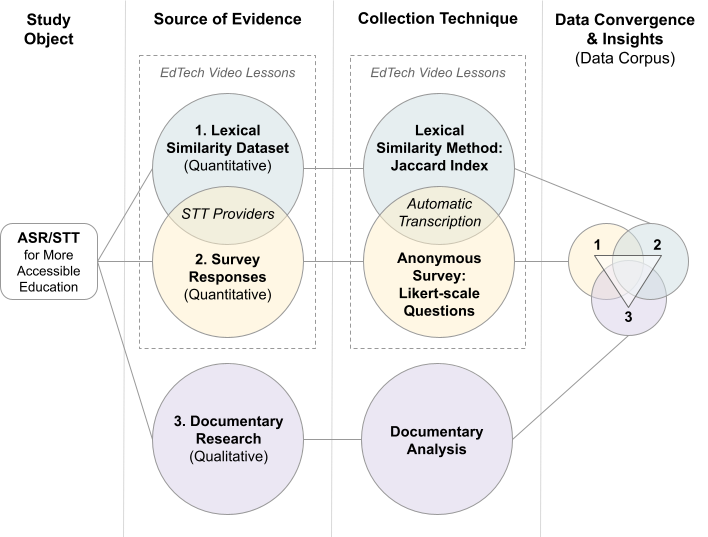
\includegraphics[width=0.9\textwidth]{images/chapter4-cs1-triangulation-methodology.png}
\fdireta{FalvoJr2024_FIE}
\end{figure}

Para as fontes de evidência quantitativas, similaridade léxica e respostas do \textit{Survey}, estabelecemos dois conjuntos de hipóteses que guiarão nossa análise. No nosso contexto, hipóteses compartilhadas fazem sentido porque ambas as fontes de evidência exploram as mesmas videoaulas e avaliam os mesmos provedores. Sendo assim, primeiro consideramos a comparação entre diferentes provedores de transcrição automática, independentemente do idioma. As hipóteses são formuladas da seguinte maneira:

\begin{itemize}
\item \textbf{Hipótese Nula ($H^0$)}: Não há diferença estatisticamente significativa na qualidade das transcrições automáticas entre os provedores.
\item \textbf{Hipótese Alternativa ($H^1$)}: Há uma diferença estatisticamente significativa na qualidade das transcrições automáticas entre os provedores.
\end{itemize}

Em segundo lugar, avaliamos a qualidade das transcrições automáticas considerando os idiomas Português, Inglês e Espanhol. As hipóteses são delineadas conforme segue:

\begin{itemize}
\item \textbf{Hipótese Nula ($H^0$)}: Não há diferença estatisticamente significativa na qualidade das transcrições automáticas para Português, Inglês e Espanhol entre os provedores.
\item \textbf{Hipótese Alternativa ($H^1$)}: Há uma diferença estatisticamente significativa na qualidade das transcrições automáticas para Português entre os provedores.
\item \textbf{Hipótese Alternativa ($H^2$)}: Há uma diferença estatisticamente significativa na qualidade das transcrições automáticas para Inglês entre os provedores.
\item \textbf{Hipótese Alternativa ($H^3$)}: Há uma diferença estatisticamente significativa na qualidade das transcrições automáticas para Espanhol entre os provedores.
\end{itemize}

Para a pesquisa documental, adotamos uma abordagem qualitativa para investigar de maneira mais ampla e exploratória como as tecnologias de reconhecimento de fala para transcrição automática (ASR e STT) influenciam a acessibilidade dos OAs. A questão de pesquisa que orienta nossa análise documental é:

\begin{itemize}
\item \textbf{Questão de Pesquisa}: Como as tecnologias de reconhecimento de fala (ASR/STT) podem contribuir para uma educação mais acessível?
\end{itemize}

Essa combinação de hipóteses quantitativas e uma questão de pesquisa qualitativa permite uma triangulação robusta de dados, fornecendo uma visão abrangente e multidimensional do impacto das tecnologias de ASR/STT na acessibilidade educacional. A análise das respostas do \textit{Survey}, juntamente com os métodos de similaridade léxica e a pesquisa documental, nos permitirá identificar as convergências entre nossas fontes de evidências e enriquecer as discussões, fortalecendo a validade do estudo.

Para fornecer uma visão formal, mas simplificada, deste primeiro Estudo de Caso, sintetizamos suas principais características na Tabela \autoref{tab:chapter4-cs1-summary}. Esta síntese foi elaborada seguindo as diretrizes metodológicas e as perspectivas de pesquisa descritas por \citeonline{CastroFilho2021}, garantindo uma abordagem estruturada e coerente com os padrões de pesquisa científica em informática na educação.

\begin{table}[htb]
\centering
\caption{Síntese do Estudo de Caso 1: Legendas Automáticas em Videoaulas}
\label{tab:chapter4-cs1-summary}
\begin{tabular}{|C{3cm}|m{11.75cm}|}\hline
\textbf{Objeto de Estudo} & Serviços de Reconhecimento de Fala (ASR/STT) \\\hline
\textbf{Perspectiva} & Explanatória (Explicativa) \\\hline
\textbf{Característica} & Explicação de causas ou efeitos relacionais ao fenômeno \cite{CastroFilho2021}. \\\hline
\textbf{Objetivos} & \begin{tabular}[c]{@{}m{11.75cm}@{}}1. Avaliar a qualidade das transcrições automáticas fornecidas por diferentes serviços de ASR/STT. \\ 2. Investigar a variação na qualidade das transcrições automáticas em diferentes idiomas (Português, Inglês e Espanhol). \\ 3. Explorar como as transcrições automáticas podem melhorar a acessibilidade educacional.\end{tabular} \\\hline
\textbf{Questões de Pesquisa} & Como as tecnologias de reconhecimento de fala (ASR/STT) podem contribuir para uma educação mais acessível? \\\hline
\textbf{Hipóteses} & \begin{tabular}[c]{@{}m{11.75cm}@{}}1. Existe diferença estatisticamente significativa na precisão das transcrições automáticas entre os provedores de ASR/STT. \\ 2. Existe diferença estatisticamente significativa na precisão das transcrições automáticas para Português, Inglês e Espanhol entre os provedores de ASR/STT.\end{tabular} \\\hline
\textbf{Fontes de Dados} & \begin{tabular}[c]{@{}m{11.75cm}@{}}1. Dados quantitativos de métodos de similaridade léxica (precisão). \\ 2. Respostas quantitativas de um \textit{Survey} anônimo (precisão). \\ 3. Dados qualitativos de uma pesquisa documental.\end{tabular} \\\hline
\textbf{Método de Coleta de Dados} & \begin{tabular}[c]{@{}m{11.75cm}@{}}Triangulação de Dados, com as seguintes fontes de evidência: \\ 1. Métodos de Similaridade Léxica. \\ 2. Respostas do \textit{Survey}. \\ 3. Pesquisa Documental.\end{tabular} \\\hline
\textbf{Tipo de Análise} & Mista (Quantitativa e Qualitativa) \\\hline
\end{tabular}
\end{table}

\subsection{Resultados e Discussões}

\subsubsection{Métodos de Similaridade Léxica}

Considerando nossas fontes de evidência quantitativas, usamos um \textit{dataset} projetado para avaliar a qualidade das transcrições automáticas de provedores líderes de ASR/STT (Amazon, Google, IBM, Microsoft e OpenAI) através de três métricas de similaridade léxica (CS, JI e LD). Nesse sentido, considerando as características dos dados coletados, focamos no JI devido ao seu desempenho estatístico mais robusto, sendo nossa única amostra com distribuição normal.

Lembrando que, o método de Jaccard mede a similaridade entre dois conjuntos de dados calculando o tamanho da interseção dividido pelo tamanho da união dos conjuntos de amostras. No nosso contexto, ele compara as palavras da transcrição automática com as da transcrição de referência (revisada por especialistas), proporcionando uma medida quantitativa de precisão. 

Sendo assim, vamos apresentar os resultados do JI como métrica principal de similaridade léxica para avaliar os provedores de ASR/STT. Os achados iniciais desta fonte de evidência podem ser visualizados por meio do conjunto de gráficos da \autoref{fig:chapter4-cs1-lexical-all}.

\begin{figure}[htbp]
\centering
\caption{Índice de Jaccard: Gráficos dos Provedores Sem Agrupar Por Idioma.}
\label{fig:chapter4-cs1-lexical-all}
\begin{subfigure}[b]{0.8\textwidth}
\centering
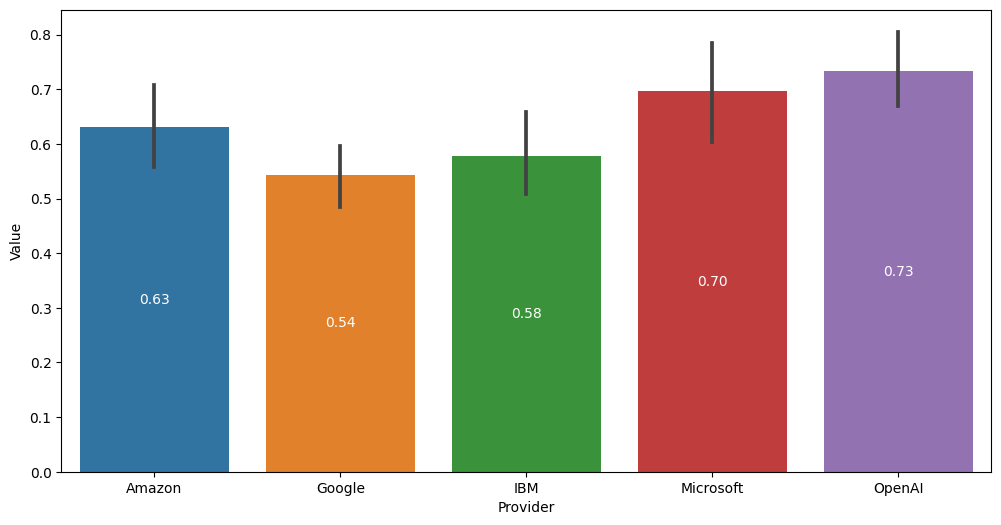
\includegraphics[width=\textwidth]{images/chapter4-cs1-lexical-all-barplot.png}
\caption{Gráfico de Barras.}
\label{fig:chapter4-cs1-lexical-all-barplot}
\end{subfigure} ~
\begin{subfigure}[b]{0.8\textwidth}
\centering
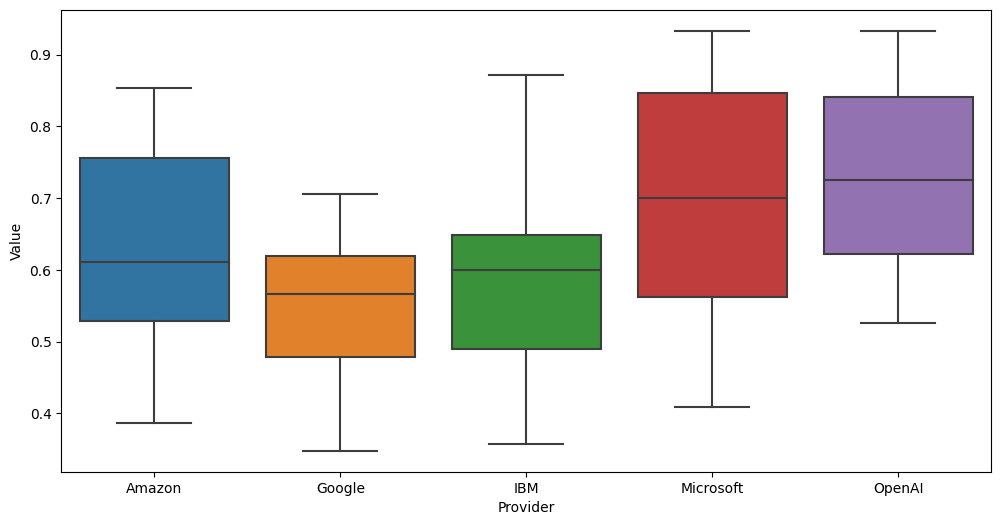
\includegraphics[width=\textwidth]{images/chapter4-cs1-lexical-all-boxplot.png}
\caption{Gráfico de Boxplot.}
\label{fig:chapter4-cs1-lexical-all-boxplot}
\end{subfigure} ~
\begin{subfigure}[b]{0.8\textwidth}
\centering
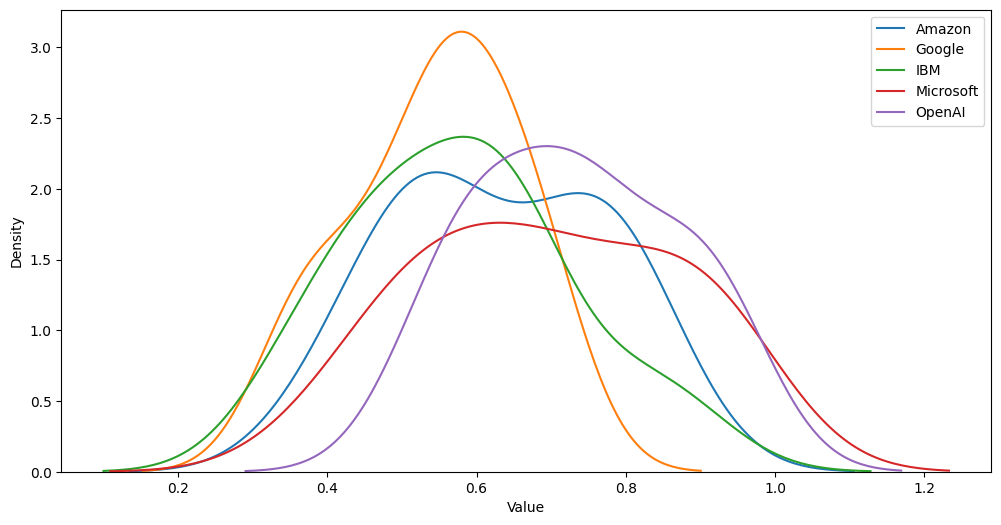
\includegraphics[width=\textwidth]{images/chapter4-cs1-lexical-all-kdeplot.png}
\caption{Gráfico KDE.}
\label{fig:chapter4-cs1-lexical-all-kdeplot}
\end{subfigure}
\fadaptada{FalvoJr2023_HICSS}
\end{figure}

A \autoref{fig:chapter4-cs1-lexical-all} inclui um Gráfico de Barras (\ref{fig:chapter4-cs1-lexical-all-barplot}) que exibe o JI médio para cada provedor, um \textit{Boxplot} (\ref{fig:chapter4-cs1-lexical-all-boxplot}) que detalha a distribuição dos dados e um Gráfico KDE (\ref{fig:chapter4-cs1-lexical-all-kdeplot}) que ilustra a densidade de probabilidade das pontuações. Essas visualizações destacaram proeminentemente a OpenAI, que demonstrou a maior pontuação, sugerindo seu desempenho superior na captura da similaridade léxica em várias aplicações de transcrição.

As análises estatísticas detalhadas na \autoref{tab:chapter4-results-ji-tests} corroboram as impressões iniciais dos gráficos. Os testes de normalidade, o \textit{Kolmogorov-Smirnov} \cite{Kolmogorov1933,Smirnov1948} e o \textit{Shapiro-Wilk} \cite{Shapiro1965}, confirmaram a distribuição normal dos dados, permitindo uma análise adicional por meio da \textit{One-Way ANOVA} \cite{Fisher1925}. 

Por sua vez, o teste de ANOVA revelou diferenças significativas entre os provedores. Portanto, as análises \textit{post-hoc} de \textit{Tukey HSD} \cite{Tukey1949} e de \textit{Bonferroni} \cite{Bonferroni1936} foram aplicadas para identificar essas diferenças explicitamente. 

\begin{table}[htb]
\centering
\caption{Testes Estatísticos do Índice de Jaccard: Provedores Sem Agrupar Por Idioma}
\label{tab:chapter4-results-ji-tests} 
\begin{tabular}{lcclc|}
\hline
\multicolumn{5}{|c|}{\textbf{Tests of Normality}} \\ \hline
\multicolumn{1}{|c|}{\multirow{2}{*}{\textbf{Test}}} & \multicolumn{2}{c|}{\textbf{Kolmogorov-Smirnov}} & \multicolumn{2}{c|}{\textbf{Shapiro-Wilk}} \\ \cline{2-5} 
\multicolumn{1}{|c|}{} & \multicolumn{1}{c|}{\textbf{Statistic}} & \multicolumn{1}{c|}{\textbf{Significance \ensuremath{(p)}}} & \multicolumn{1}{c|}{\textbf{Statistic}} & \textbf{\ensuremath{p}} \\ \hline
\multicolumn{1}{|c|}{Jaccard Index} & \multicolumn{1}{c|}{0.057} & \multicolumn{1}{c|}{\textbf{0.200}} & \multicolumn{1}{c|}{0.973} & \textbf{0.111} \\ \hline
\multicolumn{5}{|c|}{\textbf{Interpretation}} \\ \hline
\multicolumn{5}{|l|}{\begin{tabular}[c]{@{}l@{}}Kolmogorov-Smirnov: If \ensuremath{p>0.05}, sample follow the same statistical distribution.\end{tabular}} \\ \hline
\multicolumn{5}{|l|}{Shapiro-wilk: If \ensuremath{p>0.05} is normal.} \\ \hline
\multicolumn{5}{|c|}{\textbf{One-Way ANOVA (One-Way Analysis of Variance)}} \\ \hline
\multicolumn{1}{|c|}{\textbf{Test}} & \multicolumn{2}{c|}{\textbf{F}} & \multicolumn{2}{c|}{\textbf{\ensuremath{p}}} \\ \hline
\multicolumn{1}{|c|}{Jaccard Index} & \multicolumn{2}{c|}{4.562} & \multicolumn{2}{c|}{\textbf{0.002}} \\ \hline
\multicolumn{5}{|c|}{\textbf{Interpretation}} \\ \hline
\multicolumn{5}{|l|}{\begin{tabular}[c]{@{}l@{}}If \ensuremath{p<0.05}, there are significant differences between at least two groups.\end{tabular}} \\ \hline
\multicolumn{5}{|c|}{\textbf{Tukey HSD (Honest Significant Difference)}} \\ \hline
\multicolumn{3}{|l|}{\textbf{Providers (Groups from 1 to 5)}} & \multicolumn{2}{c|}{\textbf{\ensuremath{p}}} \\ \hline
\multicolumn{3}{|l|}{OpenAI (Group 5) to Google (Group 2)} & \multicolumn{2}{c|}{\textbf{0.005}} \\ \hline
\multicolumn{3}{|l|}{OpenAI (Group 5) to IBM (Group 3)} & \multicolumn{2}{c|}{\textbf{0.032}} \\ \hline
\multicolumn{3}{|l|}{Microsoft (Group 4) to Google (Group 2)} & \multicolumn{2}{c|}{\textbf{0.037}} \\ \hline
\multicolumn{5}{|c|}{\textbf{Interpretation}} \\ \hline
\multicolumn{5}{|l|}{\begin{tabular}[c]{@{}l@{}}If \ensuremath{p<>0} and \ensuremath{p<0.05}, there is a significant difference among the groups.\end{tabular}} \\ \hline
\multicolumn{5}{|c|}{\textbf{Bonferroni}} \\ \hline
\multicolumn{3}{|l|}{\textbf{Providers (Groups from 1 to 5)}} & \multicolumn{2}{c|}{\textbf{\ensuremath{p}}} \\ \hline
\multicolumn{3}{|l|}{OpenAI (Group 5) to Google (Group 2)} & \multicolumn{2}{c|}{\textbf{0.006}} \\ \hline
\multicolumn{3}{|l|}{OpenAI (Group 5) to IBM (Group 3)} & \multicolumn{2}{c|}{\textbf{0.041}} \\ \hline
\multicolumn{3}{|l|}{Microsoft (Group 4) to Google (Group 2)} & \multicolumn{2}{c|}{\textbf{0.047}} \\ \hline
\multicolumn{5}{|c|}{\textbf{Interpretation}} \\ \hline
\multicolumn{5}{|l|}{\begin{tabular}[c]{@{}l@{}}If the adjusted \ensuremath{p~(\alpha'=\alpha/n)}, where n is the number of comparisons, is \ensuremath{<0.05},\\then there is a statistical difference among the groups.\end{tabular}} \\ \hline
\end{tabular}
\fadaptada{FalvoJr2023_HICSS}
\end{table}

Adicionalmente, tendo em vista nossos dois conjuntos de hipóteses de pesquisa, as análises foram estendidas para avaliar o desempenho dos provedores em múltiplos idiomas: Português, Inglês e Espanhol (\autoref{fig:chapter4-cs1-lexical-by-lang-barplot}). Esta segmentação linguística revelou disparidades de precisão persistentes, que são críticas para aplicações globais que dependem de transcrições automáticas confiáveis em várias línguas.

\begin{figure}[htb]
\centering
\caption{Índice de Jaccard: Gráfico dos Provedores Agrupados Por Idioma.}
\label{fig:chapter4-cs1-lexical-by-lang-barplot}
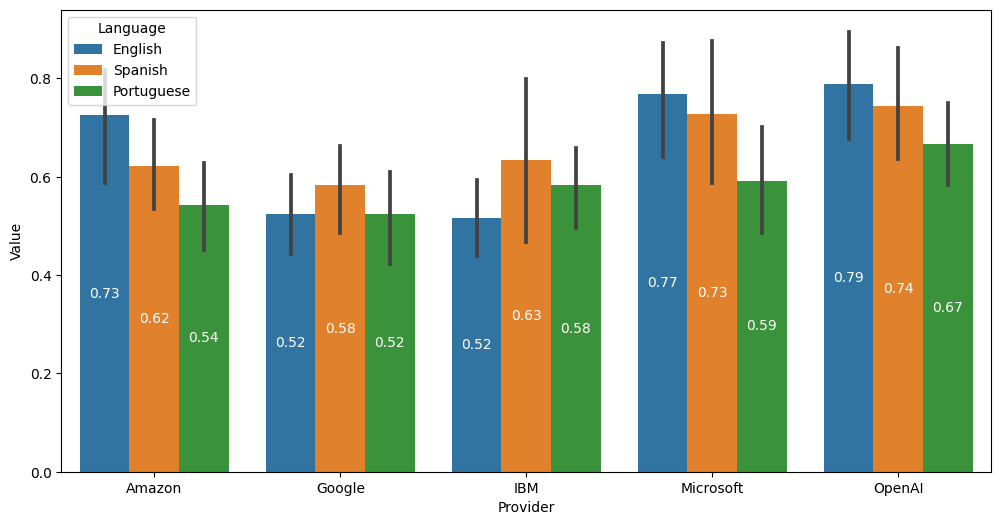
\includegraphics[width=0.9\textwidth]{images/chapter4-cs1-lexical-by-lang-barplot.png}
\fadaptada{FalvoJr2023_HICSS}
\end{figure}

Como resultado, foram identificadas diferenças estatisticamente significativas entre a OpenAI quando comparada com Google e IBM, além da Microsoft quando comparada ao Google. Essas diferenças evidenciam uma variabilidade na eficiência dos provedores ao lidar com a similaridade léxica em diferentes contextos de transcrição automática, sugerindo uma superioridade da OpenAI e da Microsoft tendo em vista suas medidas de Jaccard.

As avaliações estatísticas correspondentes (\autoref{tab:chapter4-results-ji-by-lang-tests}) incluíram testes de normalidade e \textit{One-Way ANOVA} para cada idioma. Os resultados destacaram diferenças significativas em como os provedores geram transcrições automáticas em inglês. Disparidades específicas entre provedores foram detalhadas através de análises \textit{post-hoc}, como \textit{Tukey HSD} e \textit{Bonferroni} para o idioma inglês, indicando que o desempenho pode variar significativamente dependendo do idioma das transcrições.

\begin{table}[htb]
\centering
\caption{Testes Estatísticos do Índice de Jaccard: Provedores Agrupados Por Idioma}
\label{tab:chapter4-results-ji-by-lang-tests} 
\begin{tabular}{|ccccc|}
\hline
\multicolumn{5}{|c|}{\textbf{Tests of Normality}} \\ \hline
\multicolumn{1}{|c|}{\multirow{2}{*}{\textbf{Test}}} & \multicolumn{2}{c|}{\textbf{Kolmogorov-Smirnov}} & \multicolumn{2}{c|}{\textbf{Shapiro-Wilk}} \\ \cline{2-5} 
\multicolumn{1}{|c|}{} & \multicolumn{1}{c|}{\textbf{Statistic}} & \multicolumn{1}{c|}{\textbf{Significance \ensuremath{(p)}}} & \multicolumn{1}{c|}{\textbf{Statistic}} & \textbf{\ensuremath{p}} \\ \hline
\multicolumn{1}{|c|}{EN} & \multicolumn{1}{c|}{0.121} & \multicolumn{1}{c|}{\textbf{0.200}} & \multicolumn{1}{c|}{0.961} & \textbf{0.427} \\ \hline
\multicolumn{1}{|c|}{PT} & \multicolumn{1}{c|}{0.114} & \multicolumn{1}{c|}{\textbf{0.200}} & \multicolumn{1}{c|}{0.942} & \textbf{0.169} \\ \hline
\multicolumn{1}{|c|}{ES} & \multicolumn{1}{c|}{0.951} & \multicolumn{1}{c|}{\textless 0.001} & \multicolumn{1}{c|}{0.951} & \textbf{0.264} \\ \hline
\multicolumn{5}{|c|}{\textbf{One-Way ANOVA}} \\ \hline
\multicolumn{1}{|c|}{\textbf{Test}} & \multicolumn{2}{c|}{\textbf{F}} & \multicolumn{2}{c|}{\textbf{\ensuremath{p}}} \\ \hline
\multicolumn{1}{|c|}{EN} & \multicolumn{2}{c|}{4.88} & \multicolumn{2}{c|}{\textbf{0.007}} \\ \hline
\multicolumn{1}{|c|}{PT} & \multicolumn{2}{c|}{1.058} & \multicolumn{2}{c|}{0.403} \\ \hline
\multicolumn{1}{|c|}{ES} & \multicolumn{2}{c|}{0,931} & \multicolumn{2}{c|}{0,466} \\ \hline
\multicolumn{5}{|c|}{\textbf{Tukey HSD (Honest Significant Difference) - EN}} \\ \hline
\multicolumn{3}{|l|}{\textbf{Providers (Groups from 1 to 5)}} & \multicolumn{2}{c|}{\textbf{\ensuremath{p}}} \\ \hline
\multicolumn{3}{|l|}{OpenAI (Group 5) to Google (Group 2)} & \multicolumn{2}{c|}{\textbf{0.041}} \\ \hline
\multicolumn{3}{|l|}{OpenAI (Group 5) to IBM (Group 3)} & \multicolumn{2}{c|}{\textbf{0.034}} \\ \hline
\multicolumn{5}{|c|}{\textbf{Bonferroni - EN}} \\ \hline
\multicolumn{3}{|l|}{\textbf{Providers (Groups from 1 to 5)}} & \multicolumn{2}{c|}{\textbf{\ensuremath{p}}} \\ \hline
\multicolumn{3}{|l|}{OpenAI (Group 5) to IBM (Group 3)} & \multicolumn{2}{c|}{\textbf{0.047}} \\ \hline
\end{tabular}
\fadaptada{FalvoJr2023_HICSS}
\end{table}

Esses resultados destacam diferenças significativas na qualidade das transcrições automáticas dos provedores avaliados em relação à similaridade léxica. Além disso, abrem caminho para uma exploração mais aprofundada de como essas características podem impactar a experiência do usuário em várias aplicações dessas transcrições. Isso inclui a satisfação do aluno e a percepção sobre a precisão da transcrição em diferentes contextos linguísticos. Tais aspectos são discutidos na subseção seguinte com base nos resultados do \textit{Survey}.

\subsubsection{Respostas do \textit{Survey}}

Com base nos \textit{insights} do estudo de similaridade léxica, esta seção apresenta os resultados de uma pesquisa anônima baseada nas percepções dos participantes sobre a qualidade das transcrições automáticas, explorando o \textit{dataset} definido para as fontes de evidência quantitativas. 

Essa pesquisa teve como objetivo comparar os dados objetivos de similaridade léxica com as avaliações subjetivas de pessoas reais sobre a qualidade das transcrições dos diferentes provedores de serviços de ASR/STT.

Os resultados desta pesquisa foram sintetizados na \autoref{fig:chapter4-cs1-Survey-all} para ilustrar as avaliações médias e a distribuição das respostas. O Gráfico de Barras mostra as avaliações médias para cada provedor, com a OpenAI recebendo a maior pontuação, sugerindo uma preferência entre os participantes (\ref{fig:chapter4-cs1-Survey-all-barplot}). O Gráfico de Boxplot detalha a dispersão e a tendência central das avaliações para cada provedor, destacando a variação na satisfação dos usuários (\ref{fig:chapter4-cs1-Survey-all-boxplot}), enquanto o Gráfico KDE fornece uma estimativa visual da densidade da distribuição das avaliações (\ref{fig:chapter4-cs1-Survey-all-kdeplot}).

\begin{figure}[htbp]
\centering
\caption{Respostas do \textit{Survey}: Gráficos dos Provedores Sem Agrupar Por Idioma.}
\label{fig:chapter4-cs1-Survey-all}
\begin{subfigure}[b]{0.81\textwidth}
\centering
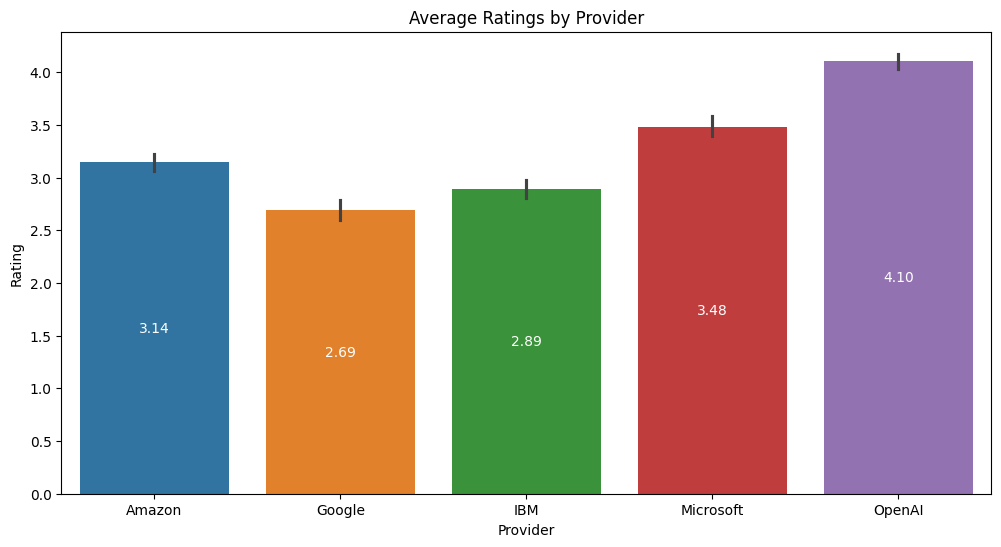
\includegraphics[width=\textwidth]{images/chapter4-cs1-survey-all-barplot.png}
\caption{Gráfico de Barras.}
\label{fig:chapter4-cs1-Survey-all-barplot}
\end{subfigure} ~
\begin{subfigure}[b]{0.81\textwidth}
\centering
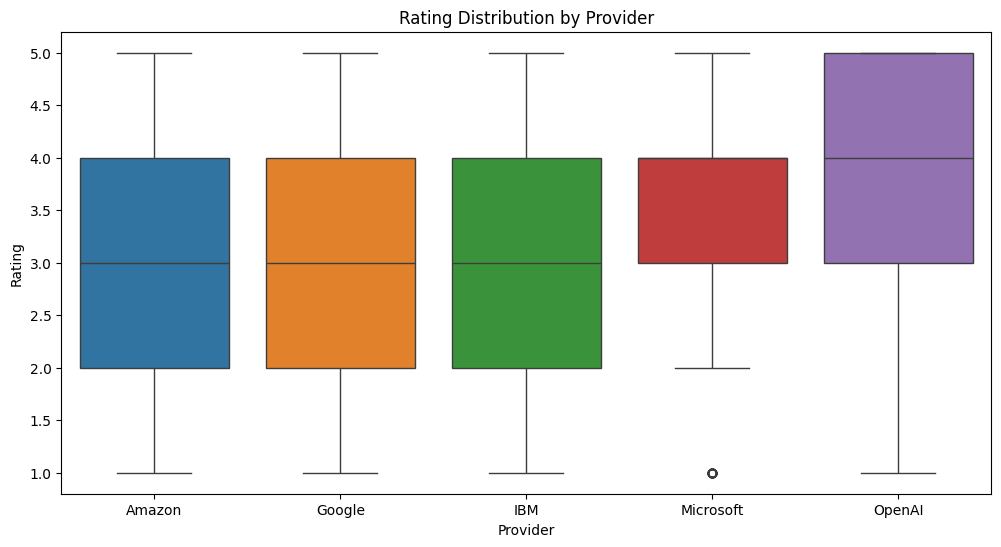
\includegraphics[width=\textwidth]{images/chapter4-cs1-survey-all-boxplot.png}
\caption{Gráfico de Boxplot.}
\label{fig:chapter4-cs1-Survey-all-boxplot}
\end{subfigure} ~
\begin{subfigure}[b]{0.81\textwidth}
\centering
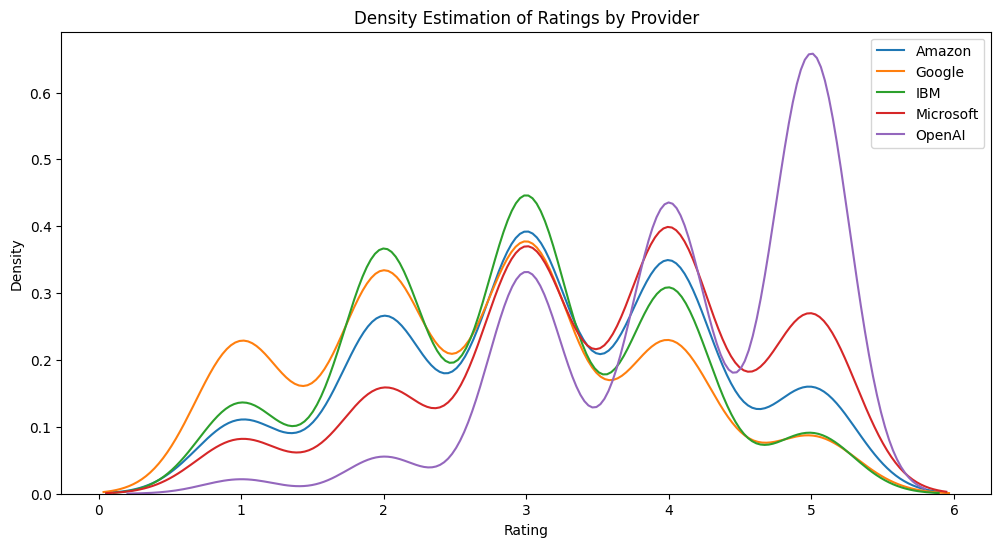
\includegraphics[width=\textwidth]{images/chapter4-cs1-survey-all-kdeplot.png}
\caption{Gráfico KDE.}
\label{fig:chapter4-cs1-Survey-all-kdeplot}
\end{subfigure}
\fadaptada{FalvoJr2024_FIE}
\end{figure}

Um gráfico adicional detalha as avaliações por idioma, indicando variações significativas na satisfação do usuário com base no idioma da transcrição automática (\autoref{fig:chapter4-cs1-Survey-by-lang-barplot}), o que pode sugerir níveis de qualidade distintos para transcrições em Português, Inglês ou Espanhol.

\begin{figure}[htb]
\centering
\caption{Respostas do \textit{Survey}: Gráfico dos Provedores Agrupados Por Idioma.}
\label{fig:chapter4-cs1-Survey-by-lang-barplot}
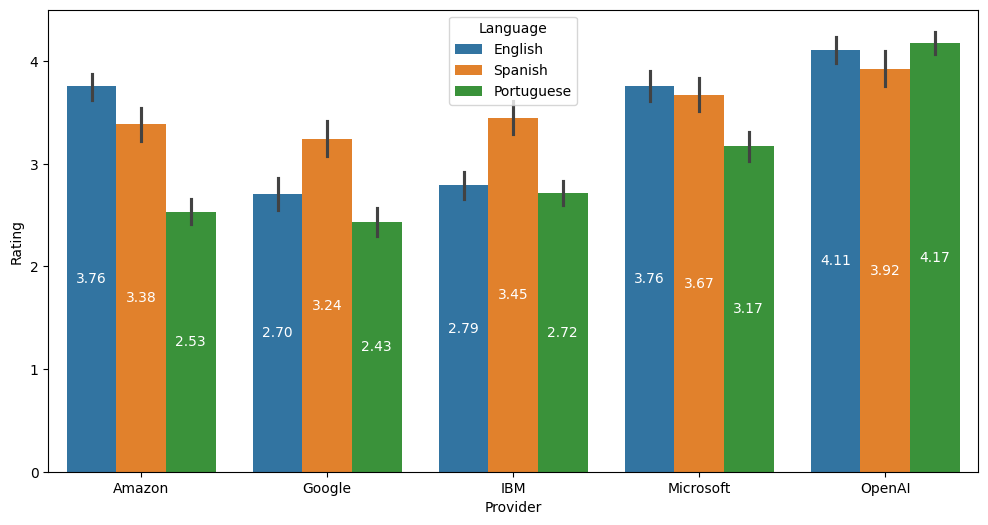
\includegraphics[width=1\textwidth]{images/chapter4-cs1-survey-by-lang-barplot.png}
\fadaptada{FalvoJr2024_FIE}
\end{figure}

As análises estatísticas, consolidadas na \autoref{tab:chapter4-results-Survey-tests}, indicaram que as respostas do \textit{Survey} não seguiram uma distribuição normal, característica confirmada pelos testes de \textit{Kolmogorov-Smirnov} \cite{Kolmogorov1933,Smirnov1948} e \textit{Shapiro-Wilk} \cite{Shapiro1965}. Por isso, se fez necessário a avaliação e aplicação de testes não paramétricos para as análises subsequentes. 

O teste de \textit{Kruskal-Wallis} \cite{Kruskal1952}, uma alternativa não paramétrica ao ANOVA, foi empregado para determinar se havia diferenças significativas nas medianas das pontuações entre os diferentes grupos. Este teste mostrou diferenças significativas entre os provedores (\ensuremath{p < 0.05}), sugerindo que as percepções dos participantes variavam significativamente dependendo do provedor.

\begin{table}[htb]
\centering
\caption{Testes Estatísticos do \textit{Survey}: Provedores Sem Agrupar Por Idioma}
\label{tab:chapter4-results-Survey-tests} 
\begin{tabular}{|lcccc|}
\hline
\multicolumn{5}{|c|}{\textbf{Tests of Normality}} \\ \hline
\multicolumn{1}{|c|}{\multirow{2}{*}{\textbf{Test}}} & \multicolumn{2}{c|}{\textbf{Kolmogorov-Smirnov}} & \multicolumn{2}{c|}{\textbf{Shapiro-Wilk}} \\ \cline{2-5} 
\multicolumn{1}{|c|}{} & \multicolumn{1}{c|}{\textbf{Statistic}} & \multicolumn{1}{c|}{\textbf{Significance \ensuremath{(p)}}} & \multicolumn{1}{c|}{\textbf{Statistic}} & \textbf{\ensuremath{p}} \\ \hline
\multicolumn{1}{|c|}{Survey Responses} & \multicolumn{1}{c|}{0.887} & \multicolumn{1}{c|}{\textless 0.001} & \multicolumn{1}{c|}{0.973} & \textless 0.001 \\ \hline
\multicolumn{5}{|c|}{\textbf{Interpretation}} \\ \hline
\multicolumn{5}{|l|}{\begin{tabular}[c]{@{}l@{}}Kolmogorov-Smirnov: If \ensuremath{p>0.05}, sample follow the same  statistical distribution.\end{tabular}} \\ \hline
\multicolumn{5}{|l|}{Shapiro-wilk: If \ensuremath{p>0.05} is normal.} \\ \hline
\multicolumn{5}{|c|}{\textbf{Kruskal-Wallis (Non-Parametric equivalent to ANOVA)}} \\ \hline
\multicolumn{1}{|c|}{\textbf{Test}} & \multicolumn{2}{c|}{\textbf{Statistic}} & \multicolumn{2}{c|}{\textbf{\ensuremath{p}}} \\ \hline
\multicolumn{1}{|c|}{Survey Responses} & \multicolumn{2}{c|}{536.167} & \multicolumn{2}{c|}{\textbf{\textless 0.001}} \\ \hline
\multicolumn{5}{|c|}{\textbf{Interpretation}} \\ \hline
\multicolumn{5}{|l|}{\begin{tabular}[c]{@{}l@{}}If \ensuremath{p<0.05}, there are significant differences among the groups.\end{tabular}} \\ \hline
\multicolumn{5}{|c|}{\textbf{Dunn (Non-Parametric Post-Hoc equivalent to Tukey HSB)}} \\ \hline
\multicolumn{3}{|l|}{\textbf{Providers (Groups from 1 to 5)}} & \multicolumn{2}{c|}{\textbf{\ensuremath{p}}} \\ \hline
\multicolumn{3}{|l|}{Amazon (Group 1) to Google (Group 2)} & \multicolumn{2}{c|}{\textbf{\textless 0.001}} \\ \hline
\multicolumn{3}{|l|}{Amazon (Group 1) to IBM (Group 3)} & \multicolumn{2}{c|}{\textbf{\textless 0.001}} \\ \hline
\multicolumn{3}{|l|}{Amazon (Group 1) to Micorsoft (Group 4)} & \multicolumn{2}{c|}{\textbf{\textless 0.001}} \\ \hline
\multicolumn{3}{|l|}{Amazon (Group 1) to OpenAI (Group 5)} & \multicolumn{2}{c|}{\textbf{\textless 0.001}} \\ \hline
\multicolumn{3}{|l|}{Google (Group 2) to IBM (Group 3)} & \multicolumn{2}{c|}{\textbf{0.010}} \\ \hline
\multicolumn{3}{|l|}{Google (Group 2) to Microsoft (Group 4)} & \multicolumn{2}{c|}{\textbf{\textless 0.001}} \\ \hline
\multicolumn{3}{|l|}{Google (Group 2) to OpenAI (Group 5)} & \multicolumn{2}{c|}{\textbf{\textless 0.001}} \\ \hline
\multicolumn{3}{|l|}{IBM (Group 3) to Microsoft (Group 4)} & \multicolumn{2}{c|}{\textbf{\textless 0.001}} \\ \hline
\multicolumn{3}{|l|}{IBM (Group 3) to OpenAI (Group 5)} & \multicolumn{2}{c|}{\textbf{\textless 0.001}} \\ \hline
\multicolumn{3}{|l|}{Micorsoft (Group 4) to OpenAI (Group 5)} & \multicolumn{2}{c|}{\textbf{\textless 0.001}} \\ \hline
\multicolumn{5}{|c|}{\textbf{Interpretation}} \\ \hline
\multicolumn{5}{|l|}{\begin{tabular}[c]{@{}l@{}}If \ensuremath{p<0.05}, it indicates significant pairwise differences between groups.\end{tabular}} \\ \hline
\end{tabular}
\fadaptada{FalvoJr2024_FIE}
\end{table}

Dada a distribuição não normal dos dados, o teste de \textit{Dunn} \cite{Dunn1964} foi escolhido em detrimento do teste de \textit{Conover} \cite{Conover1999} para a análise \textit{post-hoc} devido às suas suposições menos rigorosas sobre a distribuição dos dados e sua capacidade de lidar efetivamente com dados que possuem \textit{outliers} (\autoref{tab:chapter4-results-Survey-tests}), embora ambos tenham produzido resultados análogos em testes informais. O teste de \textit{Dunn} comparou pares de provedores, indicando diferenças significativas entre quase todos os pares. Notavelmente, todas as comparações envolvendo OpenAI e outros provedores demonstraram diferenças significativas, sugerindo uma virtual superioridade desse provedor.

Os resultados estratificados por idioma reforçaram essas descobertas, com todos os grupos de idiomas mostrando diferenças significativas entre os provedores na forma como as transcrições automáticas foram avaliadas. Isso sugere que a qualidade percebida pelos participantes não depende apenas do provedor, mas também varia com o idioma, destacando os desafios de fornecer transcrições de alta qualidade de forma uniforme em diferentes contextos linguísticos (\autoref{tab:chapter4-results-Survey-by-lang-tests}).

\begin{table}[htb]
\centering
\caption{Testes Estatísticos do \textit{Survey}: Provedores Agrupados Por Idioma}
\label{tab:chapter4-results-Survey-by-lang-tests} 
\begin{tabular}{|lcccc|}
\hline
\multicolumn{5}{|c|}{\textbf{Tests of Normality}} \\ \hline
\multicolumn{1}{|c|}{\multirow{2}{*}{\textbf{Test}}} & \multicolumn{2}{c|}{\textbf{Kolmogorov-Smirnov}} & \multicolumn{2}{c|}{\textbf{Shapiro-Wilk}} \\ \cline{2-5} 
\multicolumn{1}{|c|}{} & \multicolumn{1}{c|}{\textbf{Statistic}} & \multicolumn{1}{c|}{\textbf{Significance \ensuremath{(p)}}} & \multicolumn{1}{c|}{\textbf{Statistic}} & \textbf{\ensuremath{p}} \\ \hline
\multicolumn{1}{|c|}{EN} & \multicolumn{1}{c|}{0.897} & \multicolumn{1}{c|}{\textless 0.001} & \multicolumn{1}{c|}{0.897} & \textless 0.001 \\ \hline
\multicolumn{1}{|c|}{PT} & \multicolumn{1}{c|}{0.847} & \multicolumn{1}{c|}{\textless 0.001} & \multicolumn{1}{c|}{0.912} & \textless 0.001 \\ \hline
\multicolumn{1}{|c|}{ES} & \multicolumn{1}{c|}{0.959} & \multicolumn{1}{c|}{\textless 0.001} & \multicolumn{1}{c|}{0.893} & \textless 0.001 \\ \hline
\multicolumn{5}{|c|}{\textbf{Kruskal-Wallis (Non-Parametric)}} \\ \hline
\multicolumn{1}{|c|}{\textbf{Test}} & \multicolumn{2}{c|}{\textbf{Statistic}} & \multicolumn{2}{c|}{\textbf{\ensuremath{p}}} \\ \hline
\multicolumn{1}{|c|}{EN} & \multicolumn{2}{c|}{244.355} & \multicolumn{2}{c|}{\textbf{\textless 0.001}} \\ \hline
\multicolumn{1}{|c|}{PT} & \multicolumn{2}{c|}{355.323} & \multicolumn{2}{c|}{\textbf{\textless 0.001}} \\ \hline
\multicolumn{1}{|c|}{ES} & \multicolumn{2}{c|}{37.615} & \multicolumn{2}{c|}{\textbf{\textless 0.001}} \\ \hline
\multicolumn{5}{|c|}{\textbf{Dunn (Non-Parametric) - EN}} \\ \hline
\multicolumn{3}{|l|}{\textbf{Providers (Groups from 1 to 5)}} & \multicolumn{2}{c|}{\textbf{\ensuremath{p}}} \\ \hline
\multicolumn{3}{|l|}{Amazon (Group 1) to Google (Group 2)} & \multicolumn{2}{c|}{\textbf{\textless 0.001}} \\ \hline
\multicolumn{3}{|l|}{Amazon (Group 1) to IBM (Group 3)} & \multicolumn{2}{c|}{\textbf{\textless 0.001}} \\ \hline
\multicolumn{3}{|l|}{Amazon (Group 1) to OpenAI (Group 5)} & \multicolumn{2}{c|}{\textbf{0.002}} \\ \hline
\multicolumn{3}{|l|}{Google (Group 2) to Microsoft (Group 4)} & \multicolumn{2}{c|}{\textbf{\textless 0.001}} \\ \hline
\multicolumn{3}{|l|}{Google (Group 2) to OpenAI (Group 5)} & \multicolumn{2}{c|}{\textbf{\textless 0.001}} \\ \hline
\multicolumn{3}{|l|}{IBM (Group 3) to Microsoft (Group 4)} & \multicolumn{2}{c|}{\textbf{\textless 0.001}} \\ \hline
\multicolumn{3}{|l|}{IBM (Group 3) to OpenAI (Group 5)} & \multicolumn{2}{c|}{\textbf{\textless 0.001}} \\ \hline
\multicolumn{3}{|l|}{Micorsoft (Group 4) to OpenAI (Group 5)} & \multicolumn{2}{c|}{\textbf{0.005}} \\ \hline
\multicolumn{5}{|c|}{\textbf{Dunn (Non-Parametric) - PT}} \\ \hline
\multicolumn{3}{|l|}{\textbf{Providers (Groups from 1 to 5)}} & \multicolumn{2}{c|}{\textbf{\ensuremath{p}}} \\ \hline
\multicolumn{3}{|l|}{Amazon (Group 1) to Microsoft (Group 4)} & \multicolumn{2}{c|}{\textbf{\textless 0.001}} \\ \hline
\multicolumn{3}{|l|}{Amazon (Group 1) to OpenAI (Group 5)} & \multicolumn{2}{c|}{\textbf{\textless 0.001}} \\ \hline
\multicolumn{3}{|l|}{Google (Group 2) to IBM (Group 3)} & \multicolumn{2}{c|}{\textbf{0.017}} \\ \hline
\multicolumn{3}{|l|}{Google (Group 2) to Microsoft (Group 4)} & \multicolumn{2}{c|}{\textbf{\textless 0.001}} \\ \hline
\multicolumn{3}{|l|}{Google (Group 2) to OpenAI (Group 5)} & \multicolumn{2}{c|}{\textbf{\textless 0.001}} \\ \hline
\multicolumn{3}{|l|}{IBM (Group 3) to Microsoft (Group 4)} & \multicolumn{2}{c|}{\textbf{\textless 0.001}} \\ \hline
\multicolumn{3}{|l|}{IBM (Group 3) to OpenAI (Group 5)} & \multicolumn{2}{c|}{\textbf{\textless 0.001}} \\ \hline
\multicolumn{3}{|l|}{Micorsoft (Group 4) to OpenAI (Group 5)} & \multicolumn{2}{c|}{\textbf{\textless 0.001}} \\ \hline
\multicolumn{5}{|c|}{\textbf{Dunn (Non-Parametric) - ES}} \\ \hline
\multicolumn{3}{|l|}{\textbf{Providers (Groups from 1 to 5)}} & \multicolumn{2}{c|}{\textbf{\ensuremath{p}}} \\ \hline
\multicolumn{3}{|l|}{Amazon (Group 1) to OpenAI (Group 5)} & \multicolumn{2}{c|}{\textbf{\textless 0.001}} \\ \hline
\multicolumn{3}{|l|}{Google (Group 2) to Microsoft (Group 4)} & \multicolumn{2}{c|}{\textbf{0.002}} \\ \hline
\multicolumn{3}{|l|}{Google (Group 2) to OpenAI (Group 5)} & \multicolumn{2}{c|}{\textbf{\textless 0.001}} \\ \hline
\multicolumn{3}{|l|}{IBM (Group 3) to OpenAI (Group 5)} & \multicolumn{2}{c|}{\textbf{\textless 0.001}} \\ \hline
\end{tabular}
\fadaptada{FalvoJr2024_FIE}
\end{table}

A análise da pesquisa efetivamente conecta as medidas objetivas de similaridade léxica e as percepções subjetivas da qualidade das transcrições. A correlação entre as pontuações de similaridade léxica e as excelentes avaliações dos participantes, particularmente para a OpenAI, ressalta a relevância prática da precisão léxica na satisfação dos usuários finais. 

Esses \textit{insights} são fundamentais para provedores que buscam otimizar seus serviços de transcrição para conteúdos educacionais, pois ilustram a importância tanto da precisão linguística quanto da percepção dos usuários finais na avaliação da qualidade das transcrições automáticas. As descobertas sugerem um roteiro para futuras melhorias e a potencial customização de serviços para atender de forma mais eficaz às diversas necessidades linguísticas.

\subsubsection{Pesquisa Documental}

Nesta fase, ampliamos nossa visão sobre as tecnologias de ASR/STT, examinando a literatura para complementar nossas descobertas quantitativas com percepções qualitativas adicionais. Esta análise documental aprofunda-se em diversos estudos que contribuíram significativamente para o campo de ASR e STT, proporcionando uma compreensão mais ampla de como essas tecnologias, impulsionadas por avanços em \textit{Machine Learning} (ML) e AI, podem melhorar a acessibilidade de OAs.

O estudo de \citeonline{Ferraro2023} apresenta uma investigação extensa sobre a transcrição de língua falada usando modelos de ML. Sua análise compara serviços de STT de código aberto e pagos, com foco na qualidade das transcrições automáticas e na diversidade dos dados de entrada. A pesquisa utiliza diversos conjuntos de dados de entrevistas, palestras e discursos, empregando métricas como a Taxa de Erro de Palavras (WER) para avaliação. O trabalho de \citeonline{Ferraro2023} fornece um ponto de referência, alternativo aos métodos de similaridade léxica, para avaliar a precisão da transcrição, estabelecendo uma base sólida para trabalhos futuros.

\citeonline{Bengesi2024} oferecem uma revisão abrangente dos avanços recentes em IAGen, destacando suas aplicações potenciais em processos automáticos de transcrição. Embora não se concentrem diretamente na conversão de fala em texto, sua exploração de modelos de ponta, incluindo Redes Adversárias Generativas (GANs), Transformadores Pré-treinados Generativos (GPT), \textit{autoencoders} e modelos de difusão, fornece uma base para entender como a IAGen pode aprimorar a precisão da transcrição.

\citeonline{Homburg2019} exploram o uso de robôs humanoides como avatares para a tradução de língua de sinais, buscando aprimorar a inclusão da comunidade surda. Diferentemente de pesquisas anteriores, que se concentravam apenas no reconhecimento da língua de sinais, este estudo adota uma abordagem inovadora ao utilizar robôs como intermediários na comunicação. Entrevistando 50 participantes surdos, eles avaliam a eficácia percebida dos robôs humanoides na tradução da língua de sinais, oferecendo \textit{insights} inovadores para soluções de acessibilidade.

\citeonline{Alshaikh2024} exploram a integração da IAGen na educação por meio do desenvolvimento e avaliação de um Assistente de Vídeo Educacional com IA. Fundamentado na Teoria Cognitiva da Aprendizagem Multimídia (CTML), seu ferramental, equipado com módulos de Transcrição, Engajamento e Reforço, utiliza tecnologias ASR para aprimorar a experiência de aprendizagem. Ao focar em experiências de aprendizagem multimodal, seu estudo demonstra o potencial das técnicas avançadas de IA, incluindo STT, para melhorar os resultados educacionais.

\citeonline{Cao2023} abordam as limitações das ferramentas tradicionais de transcrição de áudio em salas de aula ruidosas do mundo real. Sua pesquisa enfatiza o papel crucial de sistemas de aprendizagem inteligentes eficazes em ambientes colaborativos, particularmente na análise e compreensão de conversas entre alunos. Ao explorar a influência dos erros de ASR em modelos de conversação, destacam os desafios e oportunidades para melhorar a precisão do ASR em contextos educacionais.

Com base nas contribuições desses estudos, pretendemos aplicar os princípios da Teoria Fundamentada em Dados \cite{Charmaz2009} para categorizar e analisar os dados qualitativos coletados em nossa pesquisa. A Teoria Fundamentada fornece uma abordagem sistemática para explorar temas emergentes e enriquecer nossa compreensão dos fatores que influenciam a qualidade das transcrições automáticas.

Ao integrar os resultados coletados de nossas fontes de evidência, buscamos identificar padrões e \textit{insights} sobre o uso de tecnologias ASR e STT na melhoria da acessibilidade dos OAs. Para facilitar essa análise, categorizamos os achados de cada estudo dentro da Teoria Fundamentada em temas distintos, permitindo uma compreensão abrangente das implicações tecnológicas e educacionais das ferramentas ASR e STT. Essas categorias incluem:

\begin{itemize}
\item \textbf{Avaliação da Qualidade de Transcrição (AQT)}: Avaliação de desempenho e qualidade em soluções baseadas nas tecnologias de ASR e STT para tarefas de transcrição de fala. Esta categoria foca na precisão das transcrições, utilizando métricas como a Taxa de Erro de Palavras (WER) e comparações entre diferentes serviços de STT, sejam eles de código aberto ou pagos.

\item \textbf{IAGen na Educação (IAGenE)}: Exploração da integração da IAGen em contextos educacionais para aprimorar experiências de aprendizagem. Aqui, a atenção está na aplicação de técnicas de IA, como GANs, GPTs e \textit{autoencoders}, para melhorar processos educacionais, incluindo a transcrição automática de aulas e a personalização da aprendizagem.

\item \textbf{Tecnologias Assistivas (TAs)}: Investigação de abordagens inovadoras, como robôs humanoides e ferramentas de aprendizagem multimodal, para melhorar a acessibilidade para diversos alunos. Esta categoria abrange o uso de TAs para suportar a inclusão de alunos com necessidades especiais, como a tradução/sinalização de línguas de sinais.

\item \textbf{Desafios e Oportunidades (DO)}: Identificação de obstáculos e possibilidades para aprimorar a precisão e eficácia do ASR em contextos educacionais. Este tema envolve os desafios na implementação de tecnologias ASR em ambientes ruidosos e colaborativos, buscando soluções para um reconhecimento de fala assertivo mesmo em situações adversas.
\end{itemize}

Na \autoref{tab:chapter4-grounded-theory-results}, apresentamos a categorização de cada estudo dentro da Teoria Fundamentada, fornecendo uma visão detalhada dos temas abordados em cada estudo e sua relevância para nossos objetivos de pesquisa. Esta análise nos permite estabelecer conexões críticas entre as diferentes vertentes de investigação, revelando como cada estudo contribui para a compreensão das tecnologias ASR e STT em contextos educacionais.

\begin{table}
\centering
\caption{Categorização dos Artigos usando Teoria Fundamentada}
\label{tab:chapter4-grounded-theory-results} 
\begin{tabular}{|c|p{6.8cm}|p{5.7cm}|}\hline
\textbf{Categoria} & \textbf{Descrição} & \textbf{Estudos} \\ \hline
\textbf{AQT} & Avalia o desempenho e qualidade do ASR/STT em tarefas de transcrição. & \citeonline{Ferraro2023} \\ \hline
\textbf{IAGenE} & Explora a integração da IAGen em contextos educacionais. & \citeonline{Bengesi2024,Alshaikh2024} \\ \hline
\textbf{TAs} & Investiga TAs para maior inclusão e acessibilidade na educação. & \citeonline{Homburg2019,Alshaikh2024} \\ \hline
\textbf{DO} & Identifica desafios e oportunidades no ASR/STT em contextos educacionais. & \citeonline{Cao2023} \\  \hline
\end{tabular}
\fadaptada{FalvoJr2024_FIE}
\end{table}

A seguir, vamos discutir a convergência dos dados provenientes das três fontes de evidência investigadas: Métodos de Similaridade Léxica, Respostas do \textit{Survey} e Pesquisa Documental. Ao integrar essas diversas fontes, buscamos uma visão mais robusta sobre o impacto das tecnologias ASR e STT na acessibilidade e eficácia dos OAs. Esta abordagem integrada nos permitirá identificar sinergias e discrepâncias, fornecendo um panorama detalhado e multifacetado dos estados da prática e da arte.

\subsubsection{Convergência de Dados}

Esta pesquisa visa desvendar as complexidades das tecnologias ASR e STT no aprimoramento da acessibilidade dos OAs por meio da triangulação de dados de três fontes distintas. Cada fonte contribui de forma única para uma compreensão abrangente de como a transcrição automática impacta a interação dos alunos com os OAs.

Primeiramente, o uso de métodos de similaridade léxica destacou variações significativas na precisão das transcrições entre os provedores de ASR avaliados (Amazon, Google, IBM, Microsoft, OpenAI). Esses dados elucidaram não apenas as capacidades técnicas desses serviços, mas também ressaltaram as nuances linguísticas que afetam seu desempenho em diferentes idiomas \cite{FalvoJr2023_HICSS}.

Adicionalmente, o \textit{Survey} estende essa análise quantitativa incorporando as percepções dos participantes sobre a qualidade das transcrições. Nesse sentido, as respostas do \textit{Survey} se alinham em alguns aspectos aos resultados da similaridade léxica, reforçando a relevância de uma boa métrica de precisão na satisfação do usuário. No entanto, também evidenciam aspectos centrados no usuário dos serviços de ASR -- como a facilidade de compreensão e a integração com ambientes de aprendizagem -- que não são capturados por algoritmos de similaridade léxica.

Esses dados quantitativos poderosos, baseados na métrica do JI e nas respostas em escala Likert do \textit{Survey}, servem como um aspecto fundamental da nossa triangulação, proporcionando uma linha de base para avaliar a precisão e, consequentemente, a qualidade das transcrições automáticas.

Por sua vez, a pesquisa documental enriquece nossa percepção ao introduzir elementos qualitativos da literatura existente. Esta análise não apenas contextualiza os achados de nossas outras fontes de evidência, mas também explora temas mais amplos, como o impacto educacional das tecnologias de ASR/STT e seu alinhamento com os princípios de acessibilidade. Essa revisão de literatura complementar identificou lacunas e oportunidades interessantes no uso atual do STT, sugerindo áreas para trabalhos futuros tanto no campo tecnológico quanto no pedagógico.

A integração desses três conjuntos de dados -- métodos de similaridade léxica, respostas do \textit{Survey} e pesquisa documental -- proporciona uma visão holística sobre o impacto das TICs, como o ASR/STT, na educação. Essa triangulação de dados não apenas confirma a importância da precisão das transcrições, mas também revela a necessidade de uma abordagem centrada no usuário e consciente do contexto para maximizar a eficácia dessas tecnologias. Sendo assim, segue uma síntese da convergência dos dados triangulados:

\begin{itemize}

\item \textbf{Similaridade Léxica vs. Percepções dos Usuários}: Os dados de similaridade léxica revelaram que diferentes provedores de STT têm diferenças estatisticamente significativas na precisão das transcrições. Notavelmente, a OpenAI mostrou um desempenho superior (geral e por idioma) quando comparada a outros provedores de peso como Google e IBM. No entanto, os resultados do \textit{Survey}, que também focaram em avaliações quantitativas, mas usando escala Likert, indicam que a satisfação do usuário é influenciada por mais do que apenas a precisão léxica. Embora a OpenAI também tenha alcançado a maior satisfação entre os participantes, as diferenças estatísticas nas respostas do \textit{Survey} sugerem que as percepções dos usuários são influenciadas por fatores como compreensão do contexto e tolerância a erros, que não são totalmente capturados pelos métodos de similaridade léxica.

\item \textbf{\textit{Insights} Qualitativos da Pesquisa Documental}: A integração da Teoria Fundamentada \cite{Charmaz2009} na nossa análise documental permitiu uma compreensão mais profunda dos temas que afetam a qualidade das transcrições automáticas. Estudos relevantes, como os de \citeonline{Ferraro2023,Alshaikh2024}, enfatizam a importância de considerar tipos de dados diversos e ambientes de aprendizagem ao avaliar tecnologias de ASR/STT. Esses achados sugerem que a eficácia educacional das aplicações de reconhecimento de fala vai além da mera precisão da transcrição, abrangendo a facilidade de integração, as capacidades de personalização e a habilidade da tecnologia de se adaptar às necessidades educacionais diversificadas.

\item \textbf{Contexto Educacional e Acessibilidade/Inclusão}: Os dados triangulados destacam a necessidade de que as tecnologias de ASR/STT se alinhem aos princípios de acessibilidade e inclusividade. As discrepâncias entre a precisão mecânica das transcrições e a satisfação qualitativa dos usuários apontam para uma lacuna nas capacidades atuais do reconhecimento de fala. Essa lacuna indica a necessidade de os provedores inovarem além das métricas tradicionais de precisão e incorporarem \textit{feedbacks} dos usuários no desenvolvimento de soluções de transcrição mais conscientes do contexto e inclusivas.

\end{itemize}

As convergências identificadas revelam que, embora a precisão léxica das transcrições seja relevante, a satisfação do usuário e a eficácia educacional dependem também de outros fatores, como a facilidade de uso e a capacidade de integração/adaptação a contextos específicos. Este panorama multifacetado sublinha a importância de uma abordagem holística no desenvolvimento e na implementação de tecnologias ASR/STT, conforme as implicações para pesquisas futuras a seguir:

\begin{itemize}
\item \textbf{Aprimoramento do Treinamento de Modelos}: Os achados indicam o potencial de melhorar as tecnologias de ASR/STT treinando modelos em conjuntos de dados linguísticos mais diversos, o que poderia ajudar na compreensão do contexto e na redução de erros nas transcrições automáticas que afetam a satisfação dos usuários finais.

\item \textbf{Customização para Uso Educacional}: Os provedores devem considerar opções de customização que permitam às instituições educacionais adaptar as funcionalidades de ASR/STT às suas necessidades específicas. Alguns exemplos nesse sentido seriam ajustes para diferentes sotaques, dialetos e vocabulário técnico específico de cursos ou disciplinas.

\item \textbf{Abordagens de Design Centrado no Usuário}: Incorporar \textit{feedbacks} dos usuários no processo de desenvolvimento pode garantir que as futuras melhorias nas tecnologias de ASR/STT estejam mais alinhadas com as necessidades e expectativas dos usuários finais, particularmente em ambientes educacionais diversificados.

\end{itemize}

A convergência dos dados da análise léxica, dos \textit{Surveys} dos usuários e da pesquisa acadêmica pinta um quadro complexo do estado atual e do potencial das tecnologias de ASR/STT na educação. Embora avanços notáveis em precisão de transcrição tenham sido alcançados, ainda há um trabalho significativo a ser feito para realizar plenamente o potencial dessas tecnologias em melhorar a acessibilidade e inclusão educacional.

Sendo assim, pesquisas futuras podem se concentrar em fechar a lacuna entre a proficiência técnica e a satisfação do usuário, enfatizando o desenvolvimento de sistemas adaptáveis, amigáveis ao usuário e conscientes do contexto que possam suportar uma ampla gama de ambientes e necessidades de aprendizagem.

Seguindo esta linha de investigação, o próximo estudo de caso explorará a PoC implementada no primeiro estudo de caso para acelerar o desenvolvimento de um player de vídeo aderente ao conceito de Design Universal. Esta PoC se aproveita das transcrições e legendas para integrar o player com avatares de Libras baseados em texto, ampliando ainda mais a acessibilidade e a inclusão em ambientes educacionais.

\section{Estudo de Caso 2: Player com Avatar de Libras}

Nosso segundo estudo concentrou-se no desenvolvimento de um player de vídeo, projetado com base no conceito de Design Universal para criar um produto final mais flexível e acessível do ponto de vista educacional \cite{GovBr2023}. Este estudo também contou com o apoio da DIO, utilizando a API REST desenvolvida como prova de conceito no primeiro estudo de caso, facilitando o acesso às videoaulas da \textit{EdTech}. Na prática, essa integração permite que o player utilize transcrições/legendas como elementos centrais para tornar seus OAs mais inclusivos.

A relevância deste estudo está em sua capacidade de explorar a eficácia e o impacto de avatares de Libras baseados em texto na acessibilidade educacional para a comunidade surda. Para isso, conduzimos avaliações quantitativas através de um Survey com intérpretes de Libras, seguido por entrevistas qualitativas, investigando como essa solução tecnológica pode melhorar a acessibilidade a OAs audíveis.

\subsection{Prova de Conceito: Player de Vídeo com Design Universal}

A \autoref{fig:chapter4-cs2-poc-diagram} ilustra, por meio de um diagrama de sequência, a dinâmica do player de vídeo desenvolvido, que utiliza as capacidades da arquitetura \textit{Speech2Learning} para ampliar a acessibilidade de videoaulas. Esta representação demonstra como o player de vídeo promove novas formas de explorar OAs audíveis, aproveitando os metadados fornecidos pela API desenvolvida anteriormente.

\begin{figure}[htbp]
\centering
\caption{Visão 2ª Instância da \textit{Speech2Learning}: Player de Vídeo com Avatar de Libras}
\label{fig:chapter4-cs2-poc-diagram}
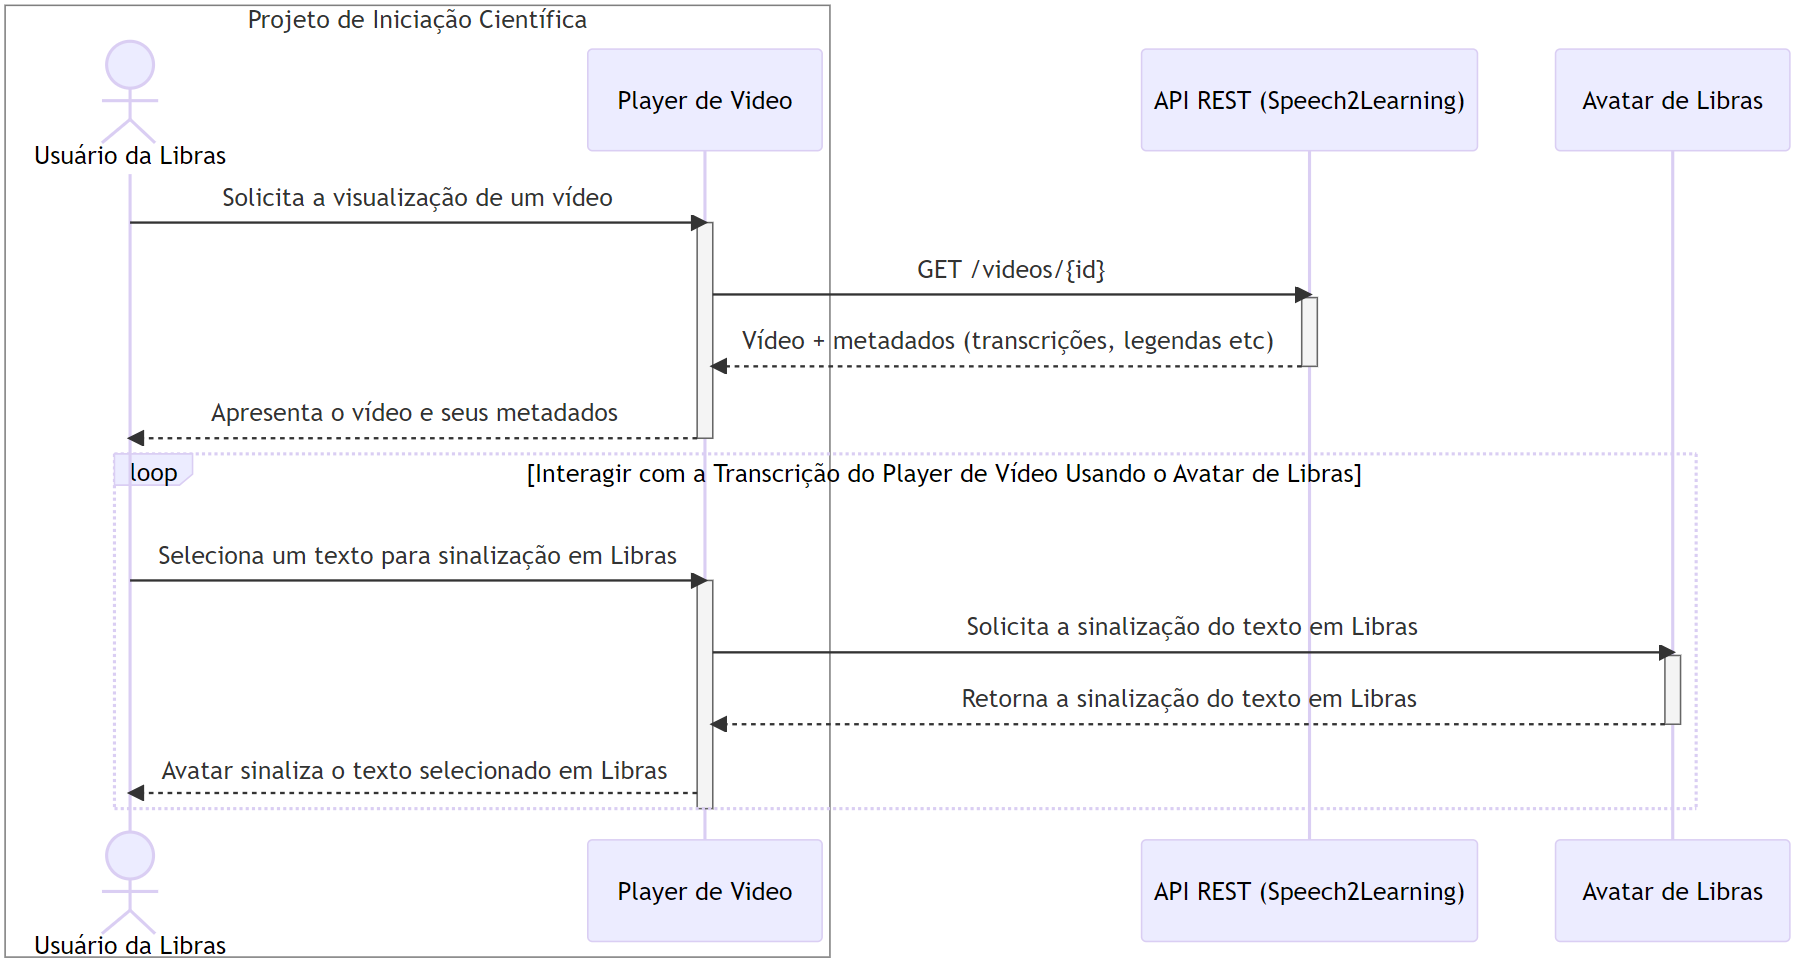
\includegraphics[width=.94\textwidth]{images/chapter4-cs2-poc-diagram.png}
\end{figure}

A integração entre o player de vídeo e a API REST ilustra a capacidade da arquitetura \textit{Speech2Learning} de fomentar ambientes educacionais mais inclusivos. Adotando esta abordagem, os desenvolvedores podem criar sistemas robustos, tecnologicamente independentes e flexíveis, capazes de atender às especificidades de cada projeto.

O objetivo central deste estudo é projetar, implementar e avaliar um player de vídeo que siga as recomendações do ``Guia de Boas Práticas para Acessibilidade Digital'' definidas por \citeonline{GovBr2023} e os princípios de Design Universal promovidos pela \citeonline{UNESCO2023}. Este player, integrado com a arquitetura \textit{Speech2Learning}, visa promover a educação inclusiva para surdos através da Libras.

Tecnicamente, o player foi implementado utilizando HTML, CSS e JavaScript de forma ``pura'' (\textit{vanilla}), ou seja, evitando bibliotecas e/ou implementações alternativas para uma solução mais padronizada e manutenível baseada na Web \cite{GovBr2023}. Os \textit{wireframes} preliminares na Figura \ref{fig:chapter4-cs2-poc-wireframes} oferecem uma visão simplificada, destacando características universais e o símbolo ``Acessível em Libras'', sublinhando o compromisso com a educação inclusiva.

\begin{figure}[htbp]
\centering
\caption{\textit{Wireframes} do Player de Vídeo Acessível (Modos Claro e Escuro)}
\label{fig:chapter4-cs2-poc-wireframes}
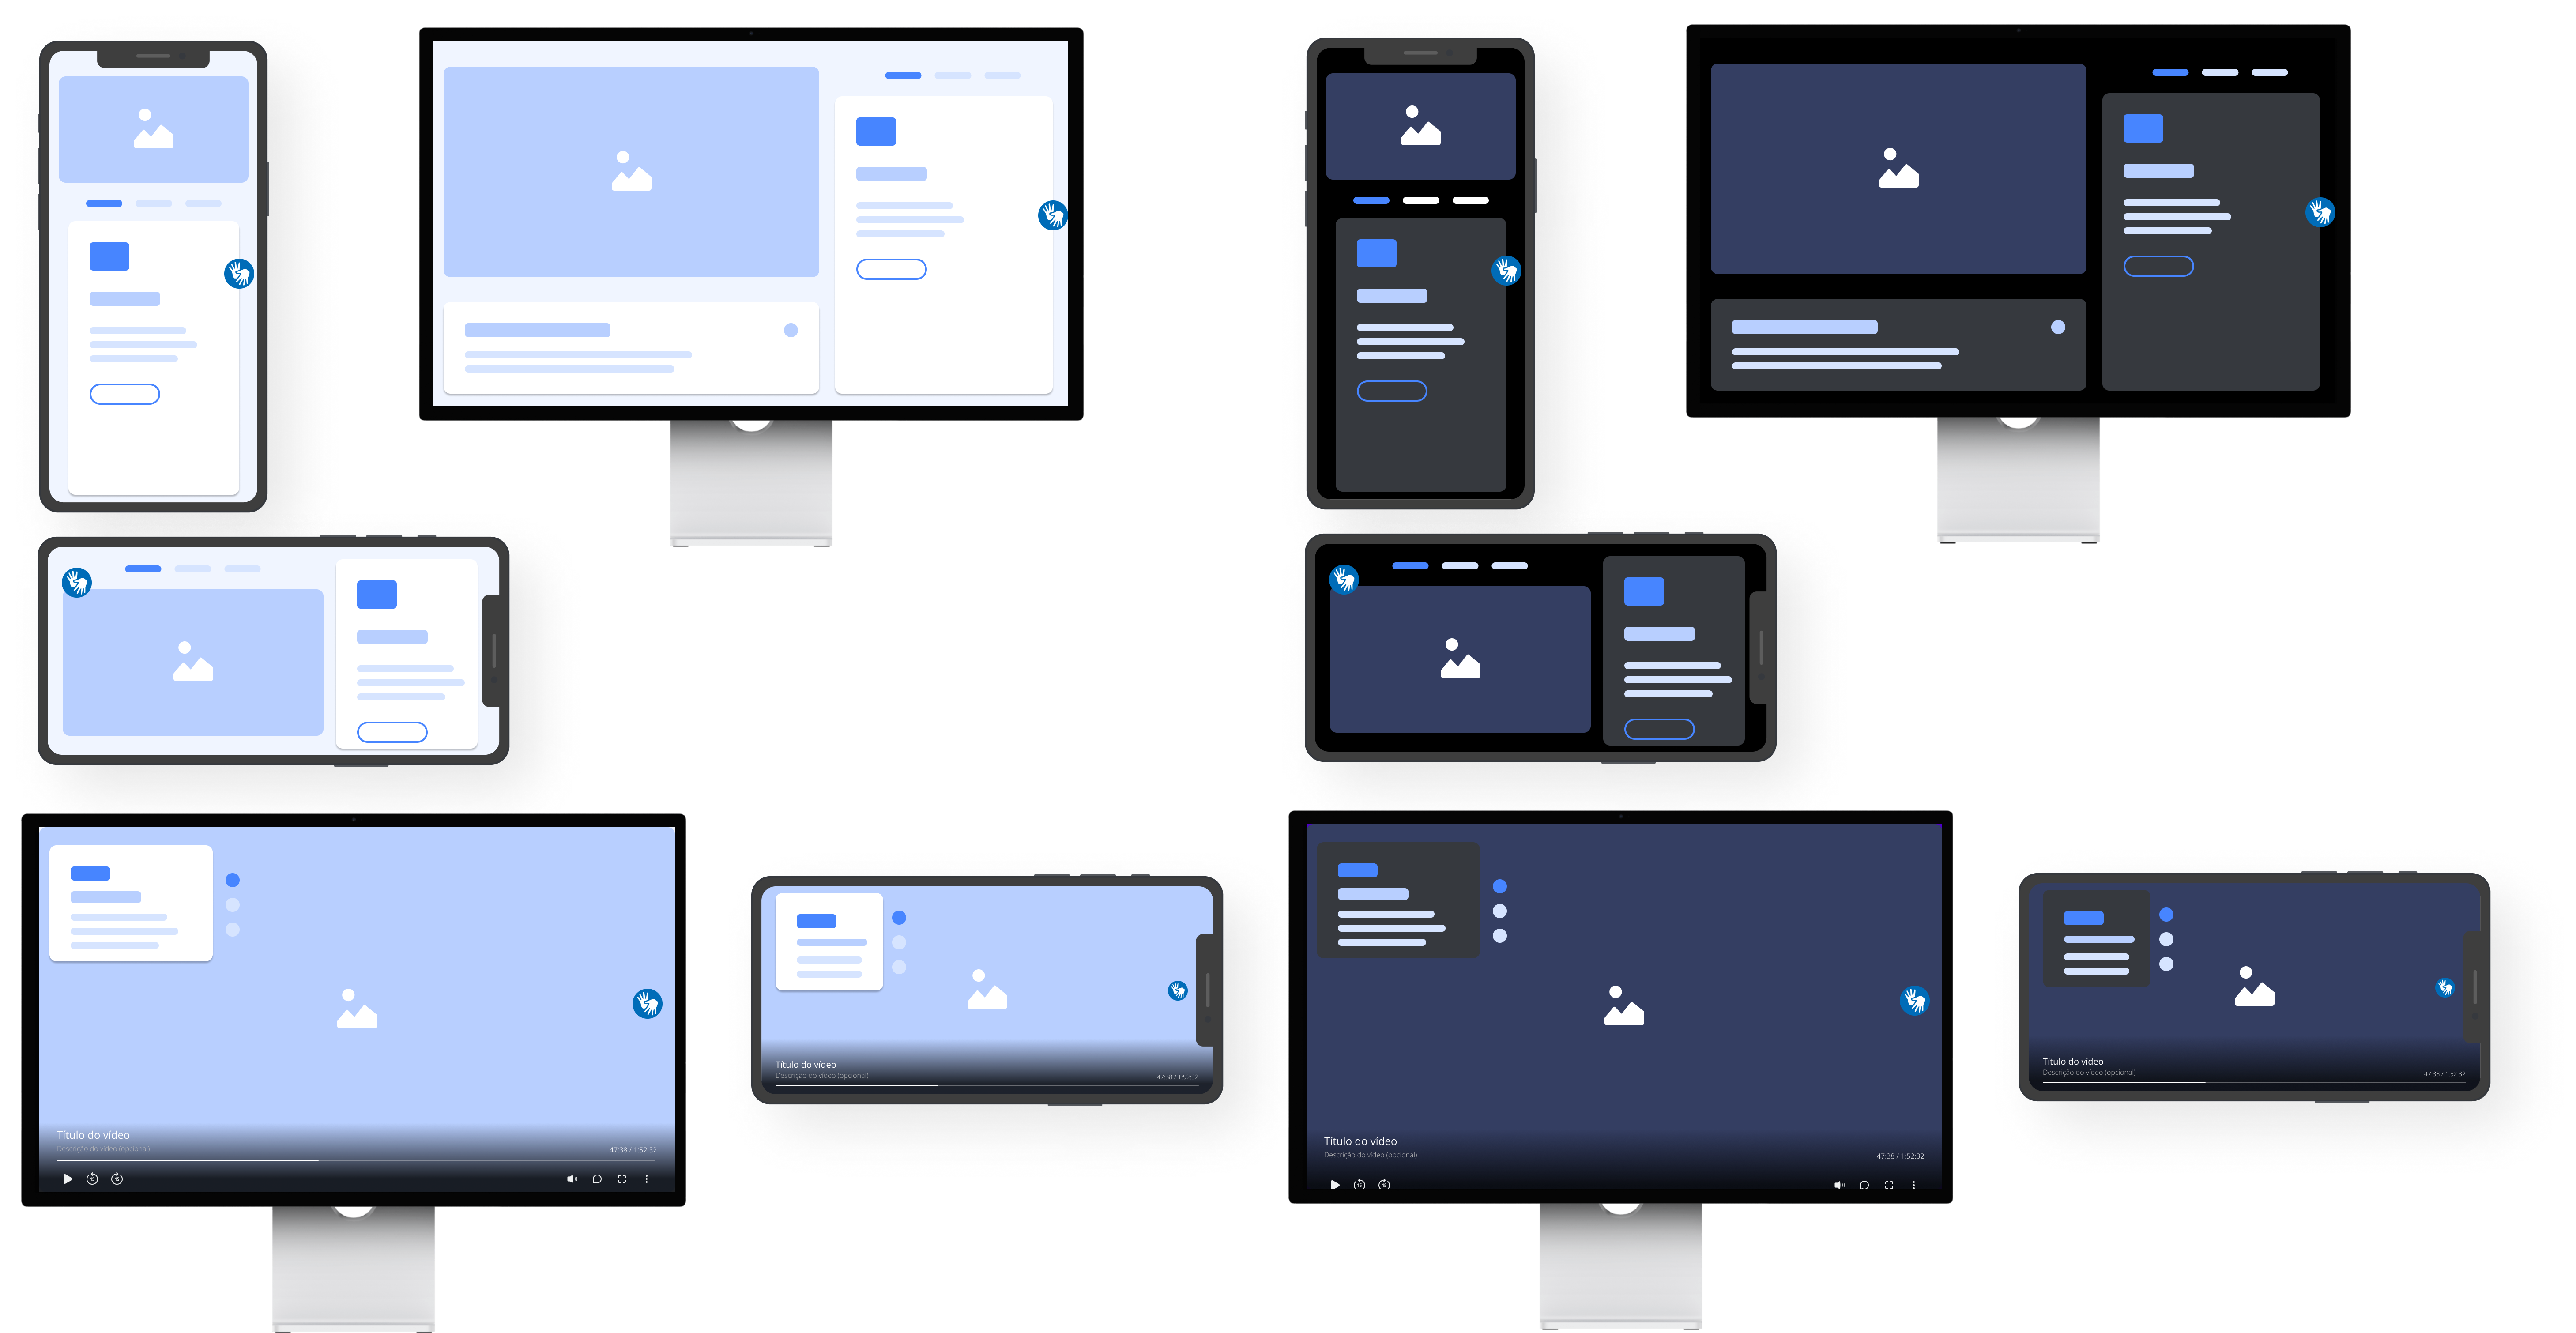
\includegraphics[width=1\textwidth]{images/chapter4-cs2-poc-wireframes.png}
\end{figure}

Em particular, esta PoC contou com dois projetos de Iniciação Científica (IC), um com foco no desenvolvimento do Design Universal da solução e outro na implementação da mesma como uma biblioteca flexível e aberta.

Sendo assim, fez-se necessário o uso de um processo de desenvolvimento de software para que as entregas fossem previsíveis e devidamente validadas. Para isso, seguimos uma metodologia ágil, com ritos simplificados e \textit{Sprints} de duas semanas.

\subsection{Metodologia}

Para investigar o impacto e a eficácia do player de vídeo com avatares de Libras baseados em texto, adotamos uma abordagem exploratória, com o objetivo de gerar conhecimento sobre um fenômeno ainda pouco conhecido \cite{CastroFilho2021}. Este estudo de caso visa atingir dois principais objetivos: (i) investigar o impacto de avatares de Libras na acessibilidade de conteúdos para surdos; e (ii) explorar a eficácia desses avatares, integrados à transcrição automática de videoaulas, para a compreensão de OAs audíveis. Para alcançar esses objetivos, formulamos a seguinte questão de pesquisa, que orienta nossa investigação:

\begin{itemize}
\item \textbf{Questão de Pesquisa}: Como as tecnologias de reconhecimento de fala (ASR/STT) podem contribuir para uma educação mais acessível para usuários da Libras?
\end{itemize}

Adotamos uma metodologia de análise mista, integrando dados quantitativos e qualitativos. Inicialmente, realizamos um Survey com todos os intérpretes da empresa QS Inclusão (\url{https://qsinclusao.com.br}), totalizando 7 participantes. No Survey, os intérpretes avaliaram quantitativamente as performances dos avatares VLibras e Hand Talk, baseados em transcrições automáticas de videoaulas. Para direcionar nossa análise quantitativa, formulamos duas hipóteses de pesquisa:

\begin{itemize}
\item \textbf{H1}: Os avatares de Libras são úteis na compreensão de OAs audíveis transcritos automaticamente.
\item \textbf{H2}: Existe diferença na qualidade de sinalização entre os avatares VLibras e Hand Talk ao utilizar transcrições automáticas.
\end{itemize}

Além do Survey, cada intérprete teve a oportunidade de agendar uma entrevista, complementando o Survey com dados qualitativos. Essas entrevistas foram planejadas para explorar profundamente as percepções e experiências dos intérpretes com o uso do player de vídeo e os avatares de Libras. A coleta de dados seguiu um protocolo semi-estruturado, garantindo que todas as áreas relevantes fossem abordadas.

A análise dos dados qualitativos foi realizada utilizando a TFD \cite{Charmaz2009}, uma metodologia que permite o desenvolvimento de teorias emergentes diretamente dos dados coletados. Este processo envolveu a codificação aberta, identificando e categorizando os principais temas nas respostas dos intérpretes de Libras. Essa abordagem assegurou que os temas emergissem naturalmente dos dados, proporcionando uma compreensão aprofundada das percepções e experiências dos participantes, sem preconceitos prévios.

Esperamos que esta segunda instância da arquitetura \textit{Speech2Learning}, através do uso de um player de vídeo acessível com avatares de Libras, melhore a acessibilidade de conteúdos educacionais para alunos surdos. Este estudo visa demonstrar que tal solução tecnológica pode:

\begin{itemize}
    \item Ampliar de maneira significativa o acesso à OAs audíveis para alunos surdos, fornecendo uma TA que potencializa a inclusão por meio do conceito de ASR, intrínseco em soluções baseadas na arquitetura \textit{Speech2Learning}.
    \item Mostrar a viabilidade e precisão dos avatares de Libras, complementando as estratégias existentes de acessibilidade presentes nas premissas de Design Universal, por exemplo.
    \item Fornecer \textit{insights} valiosos sobre as preferências dos intérpretes de Libras e suas percepções sobre a usabilidade, precisão e impacto dos avatares integrados à transcrições automáticas.
\end{itemize}

Para concluir, a síntese da \autoref{tab:chapter4-cs2-summary} resume a abordagem metodológica adotada, destacando a importância das entrevistas qualitativas para a compreensão das percepções dos intérpretes de Libras. A análise qualitativa proporcionou uma visão detalhada dos desafios e benefícios percebidos na utilização de avatares de Libras, contribuindo para o desenvolvimento de práticas pedagógicas mais inclusivas e acessíveis.

\begin{table}[htb]
\centering
\caption{Síntese do Estudo de Caso 2: Player de Vídeo com Avatar de Libras}
\label{tab:chapter4-cs2-summary}
\begin{tabular}{|C{3cm}|m{11.75cm}|}\hline
\textbf{Objeto de Estudo} & Player de Vídeo com Avatar de Libras Baseado em Texto (Transcrição Automática) \\\hline
\textbf{Perspectiva} & Exploratório \\\hline
\textbf{Característica} & Elaboração de conhecimentos ou levantamento de informação acerca do fenômeno ainda pouco conhecido \cite{CastroFilho2021}. \\\hline
\textbf{Objetivos} & \begin{tabular}[c]{@{}m{11.75cm}@{}}1. Investigar o impacto de avatares de Libras baseados em texto na acessibilidade de conteúdos para surdos. \\ 2. Explorar a eficácia de avatares de Libras integrados à transcrição automática de videoaulas para a compreensão de OAs audíveis.\end{tabular} \\\hline
\textbf{Questões de Pesquisa} & Como as tecnologias de reconhecimento de fala (ASR/STT) podem contribuir para uma educação mais acessível para usuários da Libras? \\\hline
\textbf{Hipóteses} & \begin{tabular}[c]{@{}m{11.75cm}@{}}1. Os avatares de Libras são úteis na compreensão de OAs audíveis transcritos automaticamente. \\2. Existe diferença na qualidade de sinalização entre os avatares VLibras e Hand Talk ao utilizar transcrições automáticas.\end{tabular} \\\hline
\textbf{Fontes de Dados} & Dados quantitativos do Survey e dados qualitativos de entrevistas com intérpretes de Libras. \\\hline
\textbf{Método de Coleta de Dados} & Survey e entrevistas semi-estruturadas \\\hline
\textbf{Tipo de Análise} & Mista (Quantitativa e Qualitativa) \\\hline
\end{tabular}
\end{table}

\subsection{Resultados e Discussões}

Os estudos de caso desta tese de doutorado foram aprovados pelo \sigla{CEP}{Comitê de Ética e Pesquisa}, sob o CAAE 78381524.3.0000.5390. É importante destacar que, embora ambos os estudos tenham sido descritos no projeto submetido ao CEP, o foco principal foi no Estudo de Caso 2, devido à realização de entrevistas com intérpretes de Libras e sua natureza qualitativa. Por outro lado, o Estudo de Caso 1, centrado majoritariamente em análises quantitativas da precisão de transcrições automáticas, não necessitou de uma submissão individual para avaliação ética devido às suas características.

Atualmente, as entrevistas estão sendo agendadas e conduzidas com os intérpretes de Libras da QS Inclusão. Embora os resultados ainda não tenham sido totalmente analisados e estratificados para discussões mais aprofundadas, o roteiro completo para as entrevistas com os intérpretes está disponível no \autoref{appendix:interview-form}.

Na prática, tendo em vista o nosso planejamento e previsão financeira, utilizamos apenas o \textit{VLibras} como avatar de Libras. Ele foi priorizado em detrimento ao \textit{Hand Talk} por ser gratuito, \textit{open-source} e mantido pelo governo brasileiro. Além disso, possui configurações avançadas relacionadas à regionalidade e, nos últimos anos, voltou a ser atualizado com frequência.

Algo interessante, que se alinha com esta seção, foi que tivemos a oportunidade de apresentar uma demonstração do nosso player de vídeo (\autoref{fig:chapter4-cs2-poc-demo}) no ``\textit{Workshop on Opportunities and Challenges of Generative AI in Education}'' da ``\textit{57th Hawaii International Conference on System Sciences}'' (HICSS). Seguem algumas dúvidas e \textit{feedbacks} relevantes deste evento:

\begin{figure}[htbp]
\centering
\caption{\textit{Screenshots} da Demo do Player Apresentada no HICSS.}
\label{fig:chapter4-cs2-poc-demo}
\begin{subfigure}[b]{0.83\textwidth}
\centering
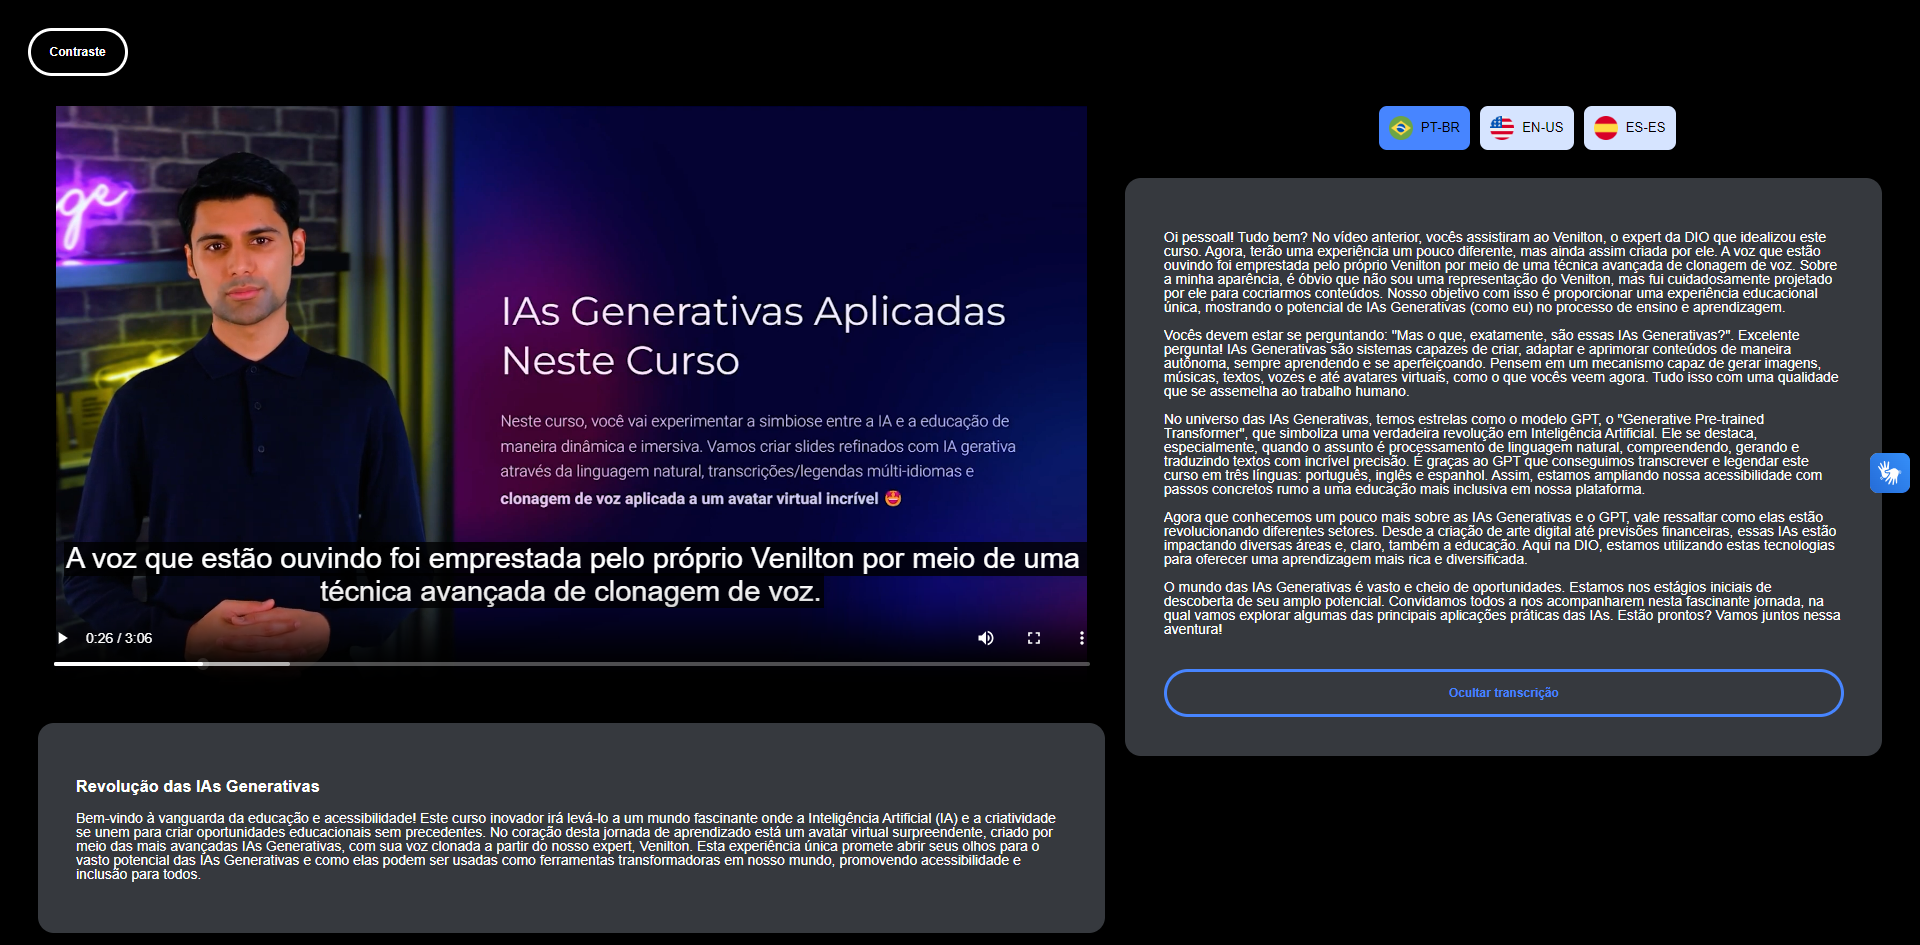
\includegraphics[width=\textwidth]{images/chapter4-cs2-poc-demo1.png}
\caption{Player de Vídeo: Transcrições e Legendas.}
\label{fig:chapter4-cs2-poc-demo1}
\end{subfigure} ~
\begin{subfigure}[b]{0.83\textwidth}
\centering
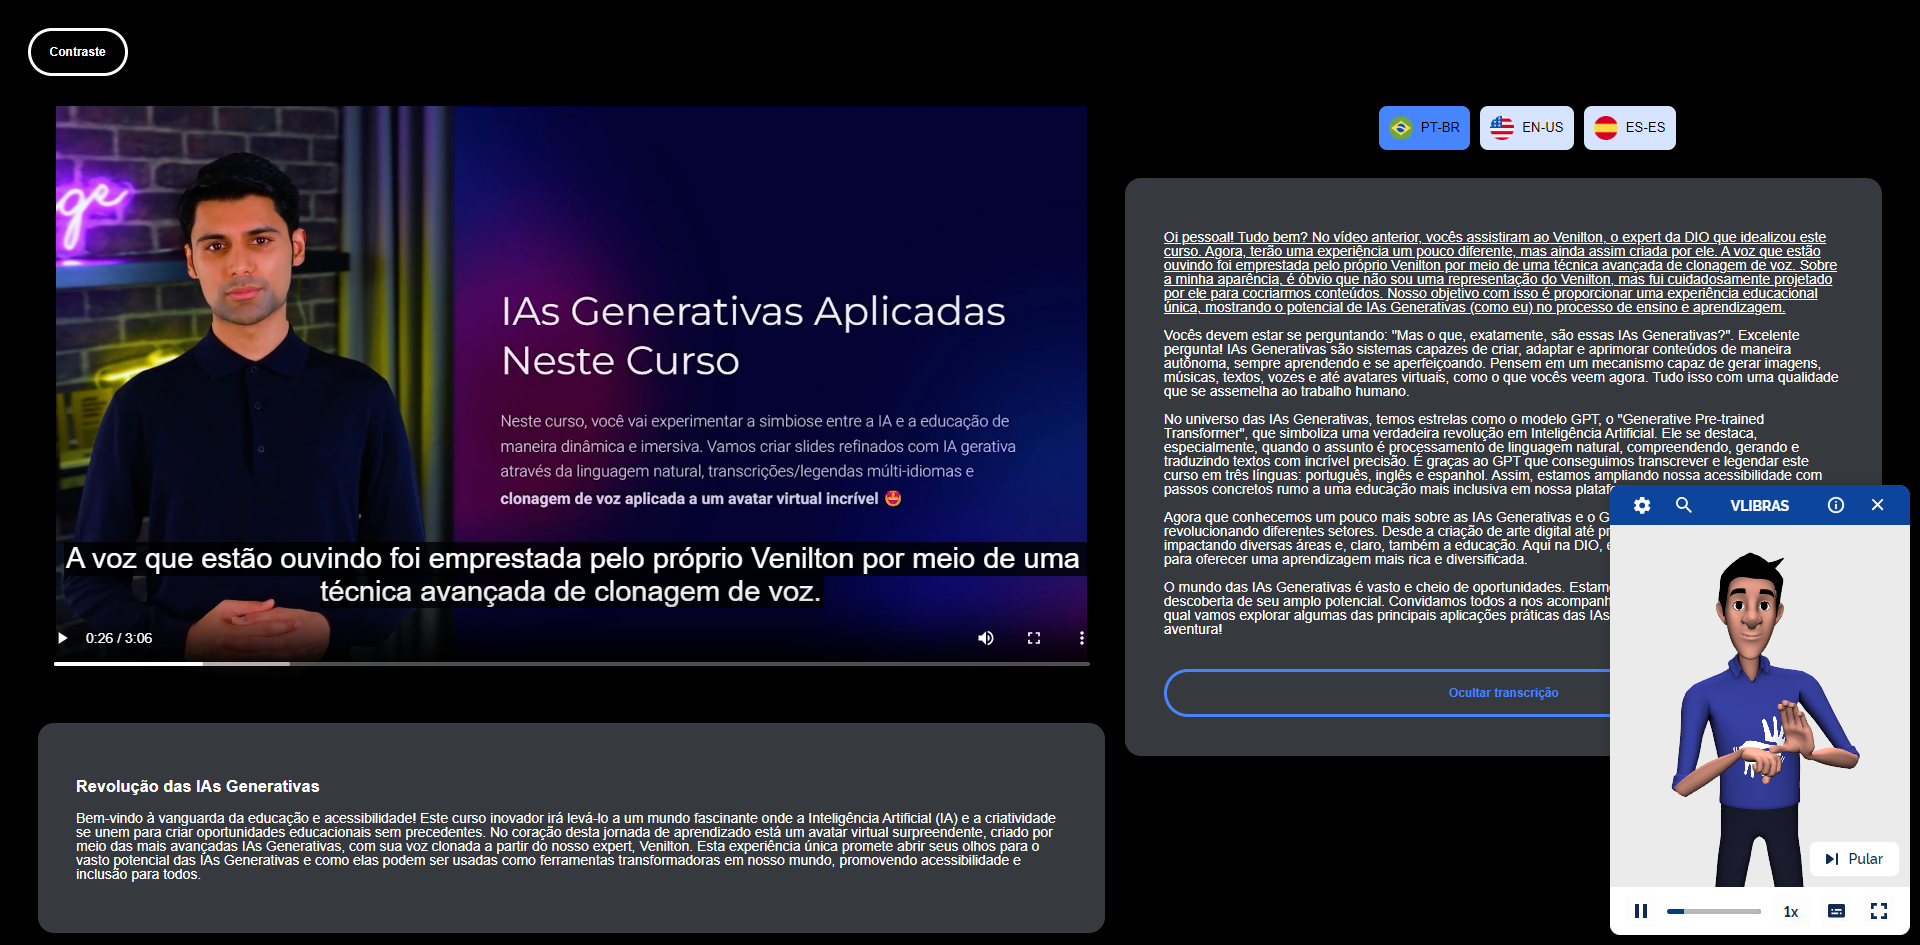
\includegraphics[width=\textwidth]{images/chapter4-cs2-poc-demo2.png}
\caption{Player de Vídeo: Avatar de Libras (VLibras) Sinalizando.}
\label{fig:chapter4-cs2-poc-demo2}
\end{subfigure} ~
\begin{subfigure}[b]{0.83\textwidth}
\centering
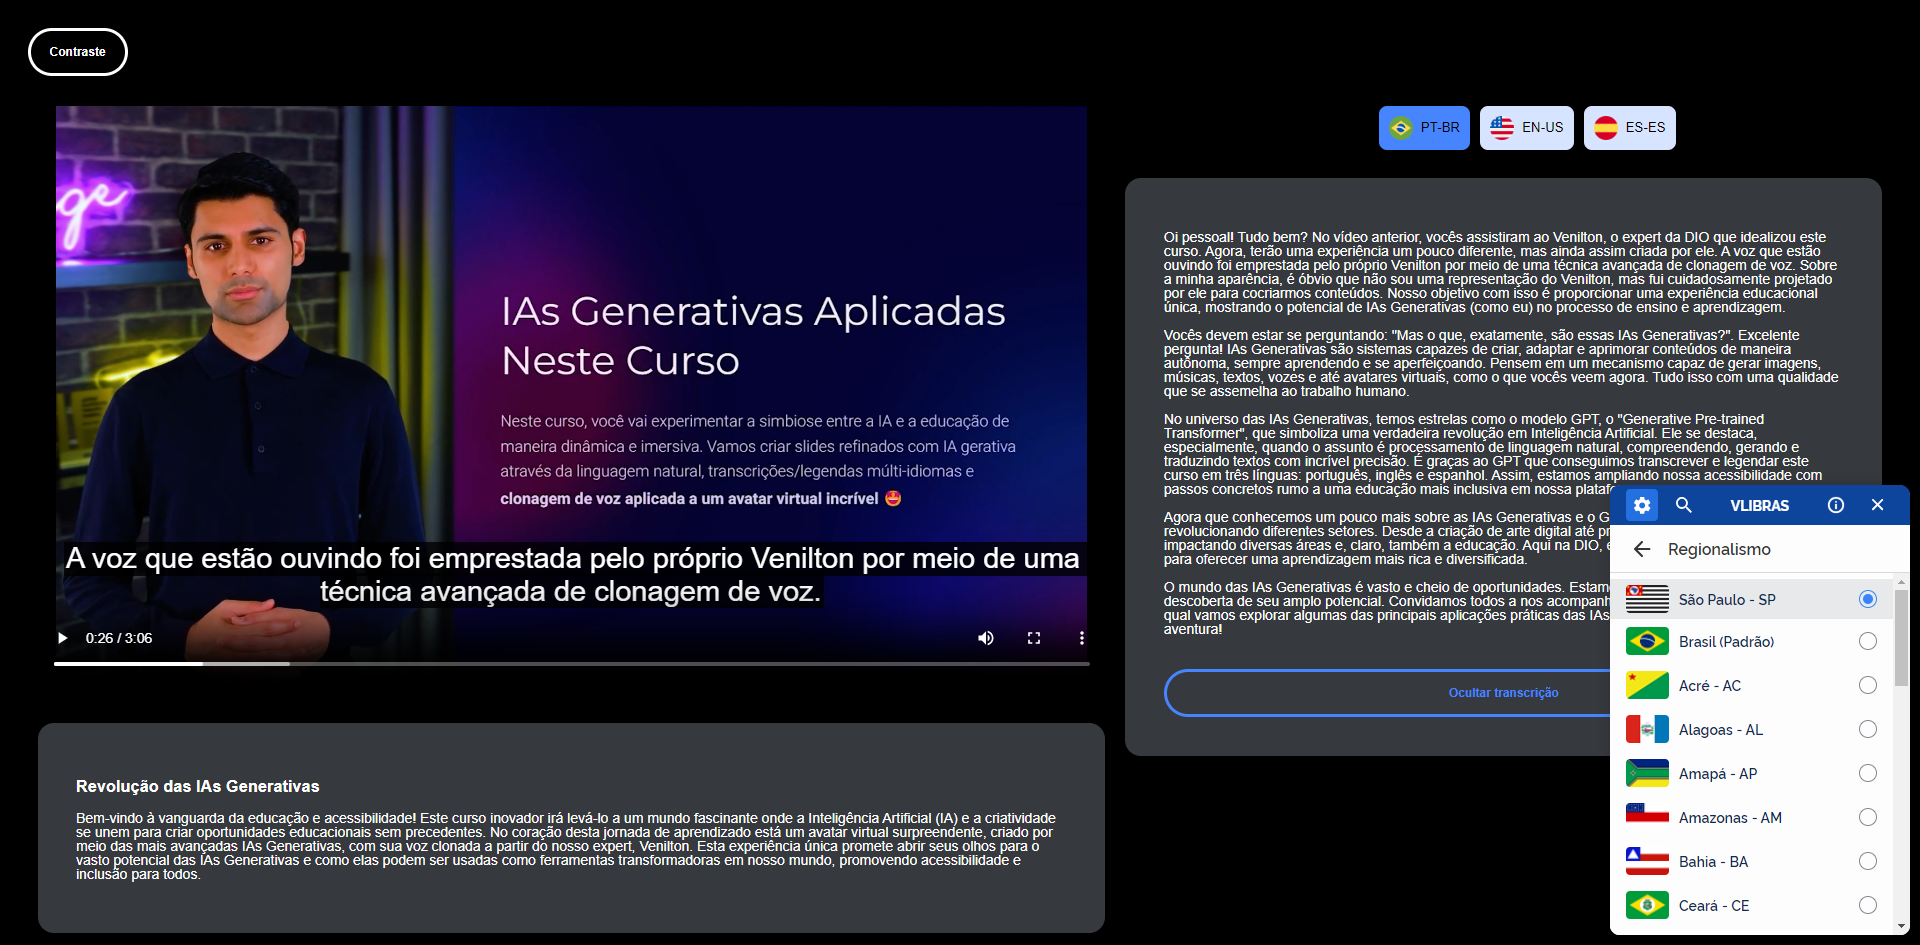
\includegraphics[width=\textwidth]{images/chapter4-cs2-poc-demo3.png}
\caption{Player de Vídeo: Avatar de Libras (VLibras) Regionalismo.}
\label{fig:chapter4-cs2-poc-demo3}
\end{subfigure}
\fautor
\end{figure}

\begin{itemize}
    \item \textbf{Como lidar com as variações regionais das próprias línguas de sinais?}
    É fundamental reconhecer a importância das regionalidades e sotaques tanto na língua falada quanto na sinalizada. A variação regional é uma característica intrínseca das línguas de sinais, que varia conforme a localização geográfica. Em nosso estudo, utilizamos o \textit{VLibras}, que possui configurações de regionalidade para cada estado do Brasil, garantindo que o avatar considere essas variações ao sinalizar. Este aspecto é crucial para a aceitação e eficácia do avatar de Libras, pois respeita as particularidades culturais e linguísticas dos usuários.
    \item \textbf{Qual seria o esforço para integrar o Player de Vídeo a avatares de outras línguas de sinais, como a ASL?}
    Nosso player foi implementado seguindo as práticas de Design Universal, que preconizam que as soluções atendam ao maior número possível de usuários. O player é, essencialmente, uma biblioteca HTML, CSS e JavaScript, garantindo que o player de vídeo HTML, bem como sua descrição, transcrições e legendas, sigam as boas práticas de semântica, estilos e interações. Dessa forma, o player não precisa "conhecer" o avatar de língua de sinais específico, pois está preparado estruturalmente para integrá-lo, facilitando a adaptação para outras línguas de sinais, como a ASL.
    \item \textbf{Como as IAGen estão ajudando no desenvolvimento de projetos relacionados à Arquitetura Speech2Learning?}
    Os modelos de ML têm evoluído consideravelmente nos últimos anos, e hoje é comum ouvirmos falar de GPT e outras siglas comuns na IA. As tecnologias de ASR e STT têm se beneficiado muito dessa revolução. O modelo de reconhecimento de fala da OpenAI, por exemplo, chamado Whisper, é baseado na ideia de \textit{Transformers}, a mesma tecnologia subjacente ao ChatGPT. Notavelmente, o Whisper se destacou em nossos testes e análises estatísticas, e foi escolhido como provedor padrão em nossa API de transcrição e legendagem de videoaulas devido à sua precisão e confiabilidade.
\end{itemize}

Em síntese, nosso estudo de caso sobre o Player de Vídeo com Avatar de Libras demonstra um avanço significativo na inclusão educacional para alunos surdos. A implementação da arquitetura \textit{Speech2Learning} com o uso de avatares de Libras, como o VLibras, potencializa a acessibilidade de conteúdos educacionais, respeitando as particularidades regionais e culturais dos usuários. A apresentação e os \textit{feedbacks} recebidos no HICSS reforçam a relevância e a aplicabilidade de nossa solução, destacando a importância de continuar explorando e aperfeiçoando tecnologias assistivas no contexto educacional.

\section{Considerações Finais}

Os dois estudos de caso apresentados nesta seção demonstram a importância e a viabilidade de utilizar tecnologias de reconhecimento de fala para promover a inclusão educacional. No primeiro estudo de caso, focado em legendas automáticas para videoaulas, comprovamos que transcrições automáticas precisas podem aumentar significativamente o potencial de acessibilidade em OAs audíveis. No segundo estudo de caso, o desenvolvimento de um player de vídeo com Design Universal, integrado com transcrições automáticas de videoaulas, mostrou-se uma solução promissora para atender às necessidades específicas da comunidade surda, oferecendo uma TA flexível e compatível com avatares de Libras baseados em texto.

Os resultados obtidos até o momento indicam que a integração de tecnologias como ASR/STT com soluções educacionais pode proporcionar uma educação mais inclusiva e acessível. A continuidade deste trabalho incluirá a análise detalhada dos dados coletados nas entrevistas com intérpretes de Libras. Além disso, futuras pesquisas poderão explorar a adaptação de avatares de outras línguas de sinais e o uso de novas tecnologias de IA para aprimorar ainda mais as soluções desenvolvidas.

Em conclusão, os estudos de caso apresentados nesta tese representam um avanço significativo na direção de uma educação verdadeiramente acessível a todos. A aplicação da arquitetura \textit{Speech2Learning} e o uso de avatares de Libras destacam-se como abordagens inovadoras e eficazes para promover a inclusão educacional, contribuindo para a construção de um ambiente educacional mais justo e igualitário.
